\documentclass[twoside]{book}

% Packages required by doxygen
\usepackage{fixltx2e}
\usepackage{calc}
\usepackage{doxygen}
\usepackage[export]{adjustbox} % also loads graphicx
\usepackage{graphicx}
\usepackage[utf8]{inputenc}
\usepackage{makeidx}
\usepackage{multicol}
\usepackage{multirow}
\PassOptionsToPackage{warn}{textcomp}
\usepackage{textcomp}
\usepackage[nointegrals]{wasysym}
\usepackage[table]{xcolor}

% Font selection
\usepackage[T1]{fontenc}
\usepackage[scaled=.90]{helvet}
\usepackage{courier}
\usepackage{amssymb}
\usepackage{sectsty}
\renewcommand{\familydefault}{\sfdefault}
\allsectionsfont{%
  \fontseries{bc}\selectfont%
  \color{darkgray}%
}
\renewcommand{\DoxyLabelFont}{%
  \fontseries{bc}\selectfont%
  \color{darkgray}%
}
\newcommand{\+}{\discretionary{\mbox{\scriptsize$\hookleftarrow$}}{}{}}

% Page & text layout
\usepackage{geometry}
\geometry{%
  a4paper,%
  top=2.5cm,%
  bottom=2.5cm,%
  left=2.5cm,%
  right=2.5cm%
}
\tolerance=750
\hfuzz=15pt
\hbadness=750
\setlength{\emergencystretch}{15pt}
\setlength{\parindent}{0cm}
\setlength{\parskip}{3ex plus 2ex minus 2ex}
\makeatletter
\renewcommand{\paragraph}{%
  \@startsection{paragraph}{4}{0ex}{-1.0ex}{1.0ex}{%
    \normalfont\normalsize\bfseries\SS@parafont%
  }%
}
\renewcommand{\subparagraph}{%
  \@startsection{subparagraph}{5}{0ex}{-1.0ex}{1.0ex}{%
    \normalfont\normalsize\bfseries\SS@subparafont%
  }%
}
\makeatother

% Headers & footers
\usepackage{fancyhdr}
\pagestyle{fancyplain}
\fancyhead[LE]{\fancyplain{}{\bfseries\thepage}}
\fancyhead[CE]{\fancyplain{}{}}
\fancyhead[RE]{\fancyplain{}{\bfseries\leftmark}}
\fancyhead[LO]{\fancyplain{}{\bfseries\rightmark}}
\fancyhead[CO]{\fancyplain{}{}}
\fancyhead[RO]{\fancyplain{}{\bfseries\thepage}}
\fancyfoot[LE]{\fancyplain{}{}}
\fancyfoot[CE]{\fancyplain{}{}}
\fancyfoot[RE]{\fancyplain{}{\bfseries\scriptsize Generated by Doxygen }}
\fancyfoot[LO]{\fancyplain{}{\bfseries\scriptsize Generated by Doxygen }}
\fancyfoot[CO]{\fancyplain{}{}}
\fancyfoot[RO]{\fancyplain{}{}}
\renewcommand{\footrulewidth}{0.4pt}
\renewcommand{\chaptermark}[1]{%
  \markboth{#1}{}%
}
\renewcommand{\sectionmark}[1]{%
  \markright{\thesection\ #1}%
}

% Indices & bibliography
\usepackage{natbib}
\usepackage[titles]{tocloft}
\setcounter{tocdepth}{3}
\setcounter{secnumdepth}{5}
\makeindex

% Hyperlinks (required, but should be loaded last)
\usepackage{ifpdf}
\ifpdf
  \usepackage[pdftex,pagebackref=true]{hyperref}
\else
  \usepackage[ps2pdf,pagebackref=true]{hyperref}
\fi
\hypersetup{%
  colorlinks=true,%
  linkcolor=blue,%
  citecolor=blue,%
  unicode%
}

% Custom commands
\newcommand{\clearemptydoublepage}{%
  \newpage{\pagestyle{empty}\cleardoublepage}%
}

\usepackage{caption}
\captionsetup{labelsep=space,justification=centering,font={bf},singlelinecheck=off,skip=4pt,position=top}

%===== C O N T E N T S =====

\begin{document}

% Titlepage & ToC
\hypersetup{pageanchor=false,
             bookmarksnumbered=true,
             pdfencoding=unicode
            }
\pagenumbering{alph}
\begin{titlepage}
\vspace*{7cm}
\begin{center}%
{\Large Cell Segmentation Project }\\
\vspace*{1cm}
{\large Generated by Doxygen 1.8.14}\\
\end{center}
\end{titlepage}
\clearemptydoublepage
\pagenumbering{roman}
\tableofcontents
\clearemptydoublepage
\pagenumbering{arabic}
\hypersetup{pageanchor=true}

%--- Begin generated contents ---
\chapter{Namespace Index}
\section{Namespace List}
Here is a list of all namespaces with brief descriptions\+:\begin{DoxyCompactList}
\item\contentsline{section}{\mbox{\hyperlink{namespace_cell_segmentation}{Cell\+Segmentation}} }{\pageref{namespace_cell_segmentation}}{}
\item\contentsline{section}{\mbox{\hyperlink{namespace_cell_segmentation_1_1settings}{Cell\+Segmentation.\+settings}} }{\pageref{namespace_cell_segmentation_1_1settings}}{}
\item\contentsline{section}{\mbox{\hyperlink{namespace_cell_segmentation_1_1urls}{Cell\+Segmentation.\+urls}} }{\pageref{namespace_cell_segmentation_1_1urls}}{}
\item\contentsline{section}{\mbox{\hyperlink{namespace_cell_segmentation_1_1wsgi}{Cell\+Segmentation.\+wsgi}} }{\pageref{namespace_cell_segmentation_1_1wsgi}}{}
\item\contentsline{section}{\mbox{\hyperlink{namespace_image_app}{Image\+App}} }{\pageref{namespace_image_app}}{}
\item\contentsline{section}{\mbox{\hyperlink{namespace_image_app_1_1admin}{Image\+App.\+admin}} }{\pageref{namespace_image_app_1_1admin}}{}
\item\contentsline{section}{\mbox{\hyperlink{namespace_image_app_1_1apps}{Image\+App.\+apps}} }{\pageref{namespace_image_app_1_1apps}}{}
\item\contentsline{section}{\mbox{\hyperlink{namespace_image_app_1_1forms}{Image\+App.\+forms}} }{\pageref{namespace_image_app_1_1forms}}{}
\item\contentsline{section}{\mbox{\hyperlink{namespace_image_app_1_1migrations}{Image\+App.\+migrations}} }{\pageref{namespace_image_app_1_1migrations}}{}
\item\contentsline{section}{\mbox{\hyperlink{namespace_image_app_1_1migrations_1_10001__initial}{Image\+App.\+migrations.\+0001\+\_\+initial}} }{\pageref{namespace_image_app_1_1migrations_1_10001__initial}}{}
\item\contentsline{section}{\mbox{\hyperlink{namespace_image_app_1_1migrations_1_10002__image__imagefile}{Image\+App.\+migrations.\+0002\+\_\+image\+\_\+imagefile}} }{\pageref{namespace_image_app_1_1migrations_1_10002__image__imagefile}}{}
\item\contentsline{section}{\mbox{\hyperlink{namespace_image_app_1_1migrations_1_10003__auto__20180818__1425}{Image\+App.\+migrations.\+0003\+\_\+auto\+\_\+20180818\+\_\+1425}} }{\pageref{namespace_image_app_1_1migrations_1_10003__auto__20180818__1425}}{}
\item\contentsline{section}{\mbox{\hyperlink{namespace_image_app_1_1migrations_1_10004__auto__20180819__1722}{Image\+App.\+migrations.\+0004\+\_\+auto\+\_\+20180819\+\_\+1722}} }{\pageref{namespace_image_app_1_1migrations_1_10004__auto__20180819__1722}}{}
\item\contentsline{section}{\mbox{\hyperlink{namespace_image_app_1_1models}{Image\+App.\+models}} }{\pageref{namespace_image_app_1_1models}}{}
\item\contentsline{section}{\mbox{\hyperlink{namespace_image_app_1_1tests}{Image\+App.\+tests}} }{\pageref{namespace_image_app_1_1tests}}{}
\item\contentsline{section}{\mbox{\hyperlink{namespace_image_app_1_1urls}{Image\+App.\+urls}} }{\pageref{namespace_image_app_1_1urls}}{}
\item\contentsline{section}{\mbox{\hyperlink{namespace_image_app_1_1views}{Image\+App.\+views}} }{\pageref{namespace_image_app_1_1views}}{}
\item\contentsline{section}{\mbox{\hyperlink{namespacemanage}{manage}} }{\pageref{namespacemanage}}{}
\item\contentsline{section}{\mbox{\hyperlink{namespacemodelo}{modelo}} }{\pageref{namespacemodelo}}{}
\end{DoxyCompactList}

\chapter{Hierarchical Index}
\section{Class Hierarchy}
This inheritance list is sorted roughly, but not completely, alphabetically\+:\begin{DoxyCompactList}
\item \contentsline{section}{Image\+App.\+forms.\+Image\+Form.\+Meta}{\pageref{class_image_app_1_1forms_1_1_image_form_1_1_meta}}{}
\item Migration\begin{DoxyCompactList}
\item \contentsline{section}{Image\+App.\+migrations.0001\+\_\+initial.Migration}{\pageref{class_image_app_1_1migrations_1_10001__initial_1_1_migration}}{}
\item \contentsline{section}{Image\+App.\+migrations.0002\+\_\+image\+\_\+imagefile.Migration}{\pageref{class_image_app_1_1migrations_1_10002__image__imagefile_1_1_migration}}{}
\item \contentsline{section}{Image\+App.\+migrations.0003\+\_\+auto\+\_\+20180818\+\_\+1425.Migration}{\pageref{class_image_app_1_1migrations_1_10003__auto__20180818__1425_1_1_migration}}{}
\item \contentsline{section}{Image\+App.\+migrations.0004\+\_\+auto\+\_\+20180819\+\_\+1722.Migration}{\pageref{class_image_app_1_1migrations_1_10004__auto__20180819__1722_1_1_migration}}{}
\end{DoxyCompactList}
\item Model\begin{DoxyCompactList}
\item \contentsline{section}{Image\+App.\+models.\+Image}{\pageref{class_image_app_1_1models_1_1_image}}{}
\end{DoxyCompactList}
\item Model\+Form\begin{DoxyCompactList}
\item \contentsline{section}{Image\+App.\+forms.\+Image\+Form}{\pageref{class_image_app_1_1forms_1_1_image_form}}{}
\end{DoxyCompactList}
\item App\+Config\begin{DoxyCompactList}
\item \contentsline{section}{Image\+App.\+apps.\+Imageapp\+Config}{\pageref{class_image_app_1_1apps_1_1_imageapp_config}}{}
\end{DoxyCompactList}
\end{DoxyCompactList}

\chapter{Class Index}
\section{Class List}
Here are the classes, structs, unions and interfaces with brief descriptions\+:\begin{DoxyCompactList}
\item\contentsline{section}{\mbox{\hyperlink{class_image_app_1_1models_1_1_image}{Image\+App.\+models.\+Image}} }{\pageref{class_image_app_1_1models_1_1_image}}{}
\item\contentsline{section}{\mbox{\hyperlink{class_image_app_1_1apps_1_1_imageapp_config}{Image\+App.\+apps.\+Imageapp\+Config}} }{\pageref{class_image_app_1_1apps_1_1_imageapp_config}}{}
\item\contentsline{section}{\mbox{\hyperlink{class_image_app_1_1forms_1_1_image_form}{Image\+App.\+forms.\+Image\+Form}} \\*Formulario para la creación de una instancia de imagen }{\pageref{class_image_app_1_1forms_1_1_image_form}}{}
\item\contentsline{section}{\mbox{\hyperlink{class_image_app_1_1forms_1_1_image_form_1_1_meta}{Image\+App.\+forms.\+Image\+Form.\+Meta}} }{\pageref{class_image_app_1_1forms_1_1_image_form_1_1_meta}}{}
\item\contentsline{section}{\mbox{\hyperlink{class_image_app_1_1migrations_1_10004__auto__20180819__1722_1_1_migration}{Image\+App.\+migrations.\+0004\+\_\+auto\+\_\+20180819\+\_\+1722.\+Migration}} }{\pageref{class_image_app_1_1migrations_1_10004__auto__20180819__1722_1_1_migration}}{}
\item\contentsline{section}{\mbox{\hyperlink{class_image_app_1_1migrations_1_10001__initial_1_1_migration}{Image\+App.\+migrations.\+0001\+\_\+initial.\+Migration}} }{\pageref{class_image_app_1_1migrations_1_10001__initial_1_1_migration}}{}
\item\contentsline{section}{\mbox{\hyperlink{class_image_app_1_1migrations_1_10003__auto__20180818__1425_1_1_migration}{Image\+App.\+migrations.\+0003\+\_\+auto\+\_\+20180818\+\_\+1425.\+Migration}} }{\pageref{class_image_app_1_1migrations_1_10003__auto__20180818__1425_1_1_migration}}{}
\item\contentsline{section}{\mbox{\hyperlink{class_image_app_1_1migrations_1_10002__image__imagefile_1_1_migration}{Image\+App.\+migrations.\+0002\+\_\+image\+\_\+imagefile.\+Migration}} }{\pageref{class_image_app_1_1migrations_1_10002__image__imagefile_1_1_migration}}{}
\item\contentsline{section}{\mbox{\hyperlink{class_kera_q_a_1_1_test_keras}{Kera\+Q\+A.\+Test\+Keras}} }{\pageref{class_kera_q_a_1_1_test_keras}}{}
\end{DoxyCompactList}

\chapter{File Index}
\section{File List}
Here is a list of all files with brief descriptions\+:\begin{DoxyCompactList}
\item\contentsline{section}{keras\+Segmentation/\mbox{\hyperlink{_kera_q_a_8py}{Kera\+Q\+A.\+py}} }{\pageref{_kera_q_a_8py}}{}
\item\contentsline{section}{keras\+Segmentation/\mbox{\hyperlink{modelo_8py}{modelo.\+py}} }{\pageref{modelo_8py}}{}
\item\contentsline{section}{pandas/\mbox{\hyperlink{manejo_archivos_c_s_v_8py}{manejo\+Archivos\+C\+S\+V.\+py}} }{\pageref{manejo_archivos_c_s_v_8py}}{}
\item\contentsline{section}{Web\+Project/\+Cell\+Segmentation/\mbox{\hyperlink{manage_8py}{manage.\+py}} }{\pageref{manage_8py}}{}
\item\contentsline{section}{Web\+Project/\+Cell\+Segmentation/\+Cell\+Segmentation/\mbox{\hyperlink{_cell_segmentation_2____init_____8py}{\+\_\+\+\_\+init\+\_\+\+\_\+.\+py}} }{\pageref{_cell_segmentation_2____init_____8py}}{}
\item\contentsline{section}{Web\+Project/\+Cell\+Segmentation/\+Cell\+Segmentation/\mbox{\hyperlink{settings_8py}{settings.\+py}} }{\pageref{settings_8py}}{}
\item\contentsline{section}{Web\+Project/\+Cell\+Segmentation/\+Cell\+Segmentation/\mbox{\hyperlink{_cell_segmentation_2urls_8py}{urls.\+py}} }{\pageref{_cell_segmentation_2urls_8py}}{}
\item\contentsline{section}{Web\+Project/\+Cell\+Segmentation/\+Cell\+Segmentation/\mbox{\hyperlink{wsgi_8py}{wsgi.\+py}} }{\pageref{wsgi_8py}}{}
\item\contentsline{section}{Web\+Project/\+Cell\+Segmentation/\+Image\+App/\mbox{\hyperlink{_image_app_2____init_____8py}{\+\_\+\+\_\+init\+\_\+\+\_\+.\+py}} }{\pageref{_image_app_2____init_____8py}}{}
\item\contentsline{section}{Web\+Project/\+Cell\+Segmentation/\+Image\+App/\mbox{\hyperlink{admin_8py}{admin.\+py}} }{\pageref{admin_8py}}{}
\item\contentsline{section}{Web\+Project/\+Cell\+Segmentation/\+Image\+App/\mbox{\hyperlink{apps_8py}{apps.\+py}} }{\pageref{apps_8py}}{}
\item\contentsline{section}{Web\+Project/\+Cell\+Segmentation/\+Image\+App/\mbox{\hyperlink{forms_8py}{forms.\+py}} }{\pageref{forms_8py}}{}
\item\contentsline{section}{Web\+Project/\+Cell\+Segmentation/\+Image\+App/\mbox{\hyperlink{models_8py}{models.\+py}} }{\pageref{models_8py}}{}
\item\contentsline{section}{Web\+Project/\+Cell\+Segmentation/\+Image\+App/\mbox{\hyperlink{tests_8py}{tests.\+py}} }{\pageref{tests_8py}}{}
\item\contentsline{section}{Web\+Project/\+Cell\+Segmentation/\+Image\+App/\mbox{\hyperlink{_image_app_2urls_8py}{urls.\+py}} }{\pageref{_image_app_2urls_8py}}{}
\item\contentsline{section}{Web\+Project/\+Cell\+Segmentation/\+Image\+App/\mbox{\hyperlink{views_8py}{views.\+py}} }{\pageref{views_8py}}{}
\item\contentsline{section}{Web\+Project/\+Cell\+Segmentation/\+Image\+App/migrations/\mbox{\hyperlink{0001__initial_8py}{0001\+\_\+initial.\+py}} }{\pageref{0001__initial_8py}}{}
\item\contentsline{section}{Web\+Project/\+Cell\+Segmentation/\+Image\+App/migrations/\mbox{\hyperlink{0002__image__imagefile_8py}{0002\+\_\+image\+\_\+imagefile.\+py}} }{\pageref{0002__image__imagefile_8py}}{}
\item\contentsline{section}{Web\+Project/\+Cell\+Segmentation/\+Image\+App/migrations/\mbox{\hyperlink{0003__auto__20180818__1425_8py}{0003\+\_\+auto\+\_\+20180818\+\_\+1425.\+py}} }{\pageref{0003__auto__20180818__1425_8py}}{}
\item\contentsline{section}{Web\+Project/\+Cell\+Segmentation/\+Image\+App/migrations/\mbox{\hyperlink{0004__auto__20180819__1722_8py}{0004\+\_\+auto\+\_\+20180819\+\_\+1722.\+py}} }{\pageref{0004__auto__20180819__1722_8py}}{}
\item\contentsline{section}{Web\+Project/\+Cell\+Segmentation/\+Image\+App/migrations/\mbox{\hyperlink{_image_app_2migrations_2____init_____8py}{\+\_\+\+\_\+init\+\_\+\+\_\+.\+py}} }{\pageref{_image_app_2migrations_2____init_____8py}}{}
\end{DoxyCompactList}

\chapter{Namespace Documentation}
\hypertarget{namespace_cell_segmentation}{}\section{Cell\+Segmentation Namespace Reference}
\label{namespace_cell_segmentation}\index{Cell\+Segmentation@{Cell\+Segmentation}}
\subsection*{Namespaces}
\begin{DoxyCompactItemize}
\item 
 \mbox{\hyperlink{namespace_cell_segmentation_1_1settings}{settings}}
\item 
 \mbox{\hyperlink{namespace_cell_segmentation_1_1urls}{urls}}
\item 
 \mbox{\hyperlink{namespace_cell_segmentation_1_1wsgi}{wsgi}}
\end{DoxyCompactItemize}

\hypertarget{namespace_cell_segmentation_1_1settings}{}\section{Cell\+Segmentation.\+settings Namespace Reference}
\label{namespace_cell_segmentation_1_1settings}\index{Cell\+Segmentation.\+settings@{Cell\+Segmentation.\+settings}}
\subsection*{Variables}
\begin{DoxyCompactItemize}
\item 
\mbox{\hyperlink{namespace_cell_segmentation_1_1settings_a354c3e9bde5b55650a0e821028acf8c2}{B\+A\+S\+E\+\_\+\+D\+IR}} = os.\+path.\+dirname(os.\+path.\+dirname(os.\+path.\+abspath(\+\_\+\+\_\+file\+\_\+\+\_\+)))
\item 
string \mbox{\hyperlink{namespace_cell_segmentation_1_1settings_a2b895f9bfae7ccf648a88cc8c31c9be0}{S\+E\+C\+R\+E\+T\+\_\+\+K\+EY}} = \textquotesingle{}0=\$\#9\$jb$^\wedge$b0w0gf!l5+ub\#ofjd3)+jjw$^\wedge$08\#1bi9$\ast$iwqur-\/a\$=\textquotesingle{}
\item 
bool \mbox{\hyperlink{namespace_cell_segmentation_1_1settings_a787047027345638dd2b9ff2df7c1dac6}{D\+E\+B\+UG}} = True
\item 
list \mbox{\hyperlink{namespace_cell_segmentation_1_1settings_aa1860414aa297264b68c5d9de3c0bb3e}{A\+L\+L\+O\+W\+E\+D\+\_\+\+H\+O\+S\+TS}} = \mbox{[}$\,$\mbox{]}
\item 
list \mbox{\hyperlink{namespace_cell_segmentation_1_1settings_a3724321f33b3f6dd16253ddddffa7d9e}{I\+N\+S\+T\+A\+L\+L\+E\+D\+\_\+\+A\+P\+PS}}
\item 
list \mbox{\hyperlink{namespace_cell_segmentation_1_1settings_a9d3647228b19e6473eb9573388ea2c04}{M\+I\+D\+D\+L\+E\+W\+A\+RE}}
\item 
string \mbox{\hyperlink{namespace_cell_segmentation_1_1settings_a0ad4c6f092c3f89b3a1cdc675dd6c1f8}{R\+O\+O\+T\+\_\+\+U\+R\+L\+C\+O\+NF}} = \textquotesingle{}Cell\+Segmentation.\+urls\textquotesingle{}
\item 
list \mbox{\hyperlink{namespace_cell_segmentation_1_1settings_a55ce1528bb9c3565782c70900d419bfb}{T\+E\+M\+P\+L\+A\+T\+ES}}
\item 
string \mbox{\hyperlink{namespace_cell_segmentation_1_1settings_a2d4d22757140f5683fc58773f5411d93}{W\+S\+G\+I\+\_\+\+A\+P\+P\+L\+I\+C\+A\+T\+I\+ON}} = \textquotesingle{}\mbox{\hyperlink{namespace_cell_segmentation_1_1wsgi_ae09dc9003f187d25053773e22660fb2a}{Cell\+Segmentation.\+wsgi.\+application}}\textquotesingle{}
\item 
dictionary \mbox{\hyperlink{namespace_cell_segmentation_1_1settings_a5cf93172a3dcca2b5cdc7f31d29eb28c}{D\+A\+T\+A\+B\+A\+S\+ES}}
\item 
list \mbox{\hyperlink{namespace_cell_segmentation_1_1settings_afdd5aa49192f7f532c0854062f6e2d16}{A\+U\+T\+H\+\_\+\+P\+A\+S\+S\+W\+O\+R\+D\+\_\+\+V\+A\+L\+I\+D\+A\+T\+O\+RS}}
\item 
string \mbox{\hyperlink{namespace_cell_segmentation_1_1settings_ac73bad9ef24ef696f2df260657a0e61c}{L\+A\+N\+G\+U\+A\+G\+E\+\_\+\+C\+O\+DE}} = \textquotesingle{}en-\/us\textquotesingle{}
\item 
string \mbox{\hyperlink{namespace_cell_segmentation_1_1settings_a1f48388d09c7f8ef633a3be8ebbc43b1}{T\+I\+M\+E\+\_\+\+Z\+O\+NE}} = \textquotesingle{}U\+TC\textquotesingle{}
\item 
bool \mbox{\hyperlink{namespace_cell_segmentation_1_1settings_af72e8510bb688294b7bd306fd168c7da}{U\+S\+E\+\_\+\+I18N}} = True
\item 
bool \mbox{\hyperlink{namespace_cell_segmentation_1_1settings_ad46d741a51b2fffd4515476c97e10bae}{U\+S\+E\+\_\+\+L10N}} = True
\item 
bool \mbox{\hyperlink{namespace_cell_segmentation_1_1settings_ac432bed0e57059113c8e1a81a5bba83a}{U\+S\+E\+\_\+\+TZ}} = True
\item 
string \mbox{\hyperlink{namespace_cell_segmentation_1_1settings_af1a1f425efd86c1b7e1148b59c82ba40}{S\+T\+A\+T\+I\+C\+\_\+\+U\+RL}} = \textquotesingle{}/static/\textquotesingle{}
\item 
string \mbox{\hyperlink{namespace_cell_segmentation_1_1settings_afcfd924da96d24487cefb726d70ba95f}{M\+E\+D\+I\+A\+\_\+\+U\+RL}} = \textquotesingle{}/media/\textquotesingle{}
\item 
\mbox{\hyperlink{namespace_cell_segmentation_1_1settings_a533430f4561df8251c4e9f96b6cf3d56}{M\+E\+D\+I\+A\+\_\+\+R\+O\+OT}} = os.\+path.\+join(\mbox{\hyperlink{namespace_cell_segmentation_1_1settings_a354c3e9bde5b55650a0e821028acf8c2}{B\+A\+S\+E\+\_\+\+D\+IR}},\textquotesingle{}media\textquotesingle{})
\end{DoxyCompactItemize}


\subsection{Variable Documentation}
\mbox{\Hypertarget{namespace_cell_segmentation_1_1settings_aa1860414aa297264b68c5d9de3c0bb3e}\label{namespace_cell_segmentation_1_1settings_aa1860414aa297264b68c5d9de3c0bb3e}} 
\index{Cell\+Segmentation\+::settings@{Cell\+Segmentation\+::settings}!A\+L\+L\+O\+W\+E\+D\+\_\+\+H\+O\+S\+TS@{A\+L\+L\+O\+W\+E\+D\+\_\+\+H\+O\+S\+TS}}
\index{A\+L\+L\+O\+W\+E\+D\+\_\+\+H\+O\+S\+TS@{A\+L\+L\+O\+W\+E\+D\+\_\+\+H\+O\+S\+TS}!Cell\+Segmentation\+::settings@{Cell\+Segmentation\+::settings}}
\subsubsection{\texorpdfstring{A\+L\+L\+O\+W\+E\+D\+\_\+\+H\+O\+S\+TS}{ALLOWED\_HOSTS}}
{\footnotesize\ttfamily list Cell\+Segmentation.\+settings.\+A\+L\+L\+O\+W\+E\+D\+\_\+\+H\+O\+S\+TS = \mbox{[}$\,$\mbox{]}}

\mbox{\Hypertarget{namespace_cell_segmentation_1_1settings_afdd5aa49192f7f532c0854062f6e2d16}\label{namespace_cell_segmentation_1_1settings_afdd5aa49192f7f532c0854062f6e2d16}} 
\index{Cell\+Segmentation\+::settings@{Cell\+Segmentation\+::settings}!A\+U\+T\+H\+\_\+\+P\+A\+S\+S\+W\+O\+R\+D\+\_\+\+V\+A\+L\+I\+D\+A\+T\+O\+RS@{A\+U\+T\+H\+\_\+\+P\+A\+S\+S\+W\+O\+R\+D\+\_\+\+V\+A\+L\+I\+D\+A\+T\+O\+RS}}
\index{A\+U\+T\+H\+\_\+\+P\+A\+S\+S\+W\+O\+R\+D\+\_\+\+V\+A\+L\+I\+D\+A\+T\+O\+RS@{A\+U\+T\+H\+\_\+\+P\+A\+S\+S\+W\+O\+R\+D\+\_\+\+V\+A\+L\+I\+D\+A\+T\+O\+RS}!Cell\+Segmentation\+::settings@{Cell\+Segmentation\+::settings}}
\subsubsection{\texorpdfstring{A\+U\+T\+H\+\_\+\+P\+A\+S\+S\+W\+O\+R\+D\+\_\+\+V\+A\+L\+I\+D\+A\+T\+O\+RS}{AUTH\_PASSWORD\_VALIDATORS}}
{\footnotesize\ttfamily list Cell\+Segmentation.\+settings.\+A\+U\+T\+H\+\_\+\+P\+A\+S\+S\+W\+O\+R\+D\+\_\+\+V\+A\+L\+I\+D\+A\+T\+O\+RS}

{\bfseries Initial value\+:}
\begin{DoxyCode}
1 =  [
2     \{
3         \textcolor{stringliteral}{'NAME'}: \textcolor{stringliteral}{'django.contrib.auth.password\_validation.UserAttributeSimilarityValidator'},
4     \},
5     \{
6         \textcolor{stringliteral}{'NAME'}: \textcolor{stringliteral}{'django.contrib.auth.password\_validation.MinimumLengthValidator'},
7     \},
8     \{
9         \textcolor{stringliteral}{'NAME'}: \textcolor{stringliteral}{'django.contrib.auth.password\_validation.CommonPasswordValidator'},
10     \},
11     \{
12         \textcolor{stringliteral}{'NAME'}: \textcolor{stringliteral}{'django.contrib.auth.password\_validation.NumericPasswordValidator'},
13     \},
14 ]
\end{DoxyCode}
\mbox{\Hypertarget{namespace_cell_segmentation_1_1settings_a354c3e9bde5b55650a0e821028acf8c2}\label{namespace_cell_segmentation_1_1settings_a354c3e9bde5b55650a0e821028acf8c2}} 
\index{Cell\+Segmentation\+::settings@{Cell\+Segmentation\+::settings}!B\+A\+S\+E\+\_\+\+D\+IR@{B\+A\+S\+E\+\_\+\+D\+IR}}
\index{B\+A\+S\+E\+\_\+\+D\+IR@{B\+A\+S\+E\+\_\+\+D\+IR}!Cell\+Segmentation\+::settings@{Cell\+Segmentation\+::settings}}
\subsubsection{\texorpdfstring{B\+A\+S\+E\+\_\+\+D\+IR}{BASE\_DIR}}
{\footnotesize\ttfamily Cell\+Segmentation.\+settings.\+B\+A\+S\+E\+\_\+\+D\+IR = os.\+path.\+dirname(os.\+path.\+dirname(os.\+path.\+abspath(\+\_\+\+\_\+file\+\_\+\+\_\+)))}

\mbox{\Hypertarget{namespace_cell_segmentation_1_1settings_a5cf93172a3dcca2b5cdc7f31d29eb28c}\label{namespace_cell_segmentation_1_1settings_a5cf93172a3dcca2b5cdc7f31d29eb28c}} 
\index{Cell\+Segmentation\+::settings@{Cell\+Segmentation\+::settings}!D\+A\+T\+A\+B\+A\+S\+ES@{D\+A\+T\+A\+B\+A\+S\+ES}}
\index{D\+A\+T\+A\+B\+A\+S\+ES@{D\+A\+T\+A\+B\+A\+S\+ES}!Cell\+Segmentation\+::settings@{Cell\+Segmentation\+::settings}}
\subsubsection{\texorpdfstring{D\+A\+T\+A\+B\+A\+S\+ES}{DATABASES}}
{\footnotesize\ttfamily dictionary Cell\+Segmentation.\+settings.\+D\+A\+T\+A\+B\+A\+S\+ES}

{\bfseries Initial value\+:}
\begin{DoxyCode}
1 =  \{
2     \textcolor{stringliteral}{'default'}: \{
3         \textcolor{stringliteral}{'ENGINE'}: \textcolor{stringliteral}{'django.db.backends.sqlite3'},
4         \textcolor{stringliteral}{'NAME'}: os.path.join(BASE\_DIR, \textcolor{stringliteral}{'db.sqlite3'}),
5     \}
6 \}
\end{DoxyCode}
\mbox{\Hypertarget{namespace_cell_segmentation_1_1settings_a787047027345638dd2b9ff2df7c1dac6}\label{namespace_cell_segmentation_1_1settings_a787047027345638dd2b9ff2df7c1dac6}} 
\index{Cell\+Segmentation\+::settings@{Cell\+Segmentation\+::settings}!D\+E\+B\+UG@{D\+E\+B\+UG}}
\index{D\+E\+B\+UG@{D\+E\+B\+UG}!Cell\+Segmentation\+::settings@{Cell\+Segmentation\+::settings}}
\subsubsection{\texorpdfstring{D\+E\+B\+UG}{DEBUG}}
{\footnotesize\ttfamily bool Cell\+Segmentation.\+settings.\+D\+E\+B\+UG = True}

\mbox{\Hypertarget{namespace_cell_segmentation_1_1settings_a3724321f33b3f6dd16253ddddffa7d9e}\label{namespace_cell_segmentation_1_1settings_a3724321f33b3f6dd16253ddddffa7d9e}} 
\index{Cell\+Segmentation\+::settings@{Cell\+Segmentation\+::settings}!I\+N\+S\+T\+A\+L\+L\+E\+D\+\_\+\+A\+P\+PS@{I\+N\+S\+T\+A\+L\+L\+E\+D\+\_\+\+A\+P\+PS}}
\index{I\+N\+S\+T\+A\+L\+L\+E\+D\+\_\+\+A\+P\+PS@{I\+N\+S\+T\+A\+L\+L\+E\+D\+\_\+\+A\+P\+PS}!Cell\+Segmentation\+::settings@{Cell\+Segmentation\+::settings}}
\subsubsection{\texorpdfstring{I\+N\+S\+T\+A\+L\+L\+E\+D\+\_\+\+A\+P\+PS}{INSTALLED\_APPS}}
{\footnotesize\ttfamily list Cell\+Segmentation.\+settings.\+I\+N\+S\+T\+A\+L\+L\+E\+D\+\_\+\+A\+P\+PS}

{\bfseries Initial value\+:}
\begin{DoxyCode}
1 =  [
2     \textcolor{stringliteral}{'django.contrib.admin'},
3     \textcolor{stringliteral}{'django.contrib.auth'},
4     \textcolor{stringliteral}{'django.contrib.contenttypes'},
5     \textcolor{stringliteral}{'django.contrib.sessions'},
6     \textcolor{stringliteral}{'django.contrib.messages'},
7     \textcolor{stringliteral}{'django.contrib.staticfiles'},
8     \textcolor{stringliteral}{'ImageApp'},
9 ]
\end{DoxyCode}
\mbox{\Hypertarget{namespace_cell_segmentation_1_1settings_ac73bad9ef24ef696f2df260657a0e61c}\label{namespace_cell_segmentation_1_1settings_ac73bad9ef24ef696f2df260657a0e61c}} 
\index{Cell\+Segmentation\+::settings@{Cell\+Segmentation\+::settings}!L\+A\+N\+G\+U\+A\+G\+E\+\_\+\+C\+O\+DE@{L\+A\+N\+G\+U\+A\+G\+E\+\_\+\+C\+O\+DE}}
\index{L\+A\+N\+G\+U\+A\+G\+E\+\_\+\+C\+O\+DE@{L\+A\+N\+G\+U\+A\+G\+E\+\_\+\+C\+O\+DE}!Cell\+Segmentation\+::settings@{Cell\+Segmentation\+::settings}}
\subsubsection{\texorpdfstring{L\+A\+N\+G\+U\+A\+G\+E\+\_\+\+C\+O\+DE}{LANGUAGE\_CODE}}
{\footnotesize\ttfamily string Cell\+Segmentation.\+settings.\+L\+A\+N\+G\+U\+A\+G\+E\+\_\+\+C\+O\+DE = \textquotesingle{}en-\/us\textquotesingle{}}

\mbox{\Hypertarget{namespace_cell_segmentation_1_1settings_a533430f4561df8251c4e9f96b6cf3d56}\label{namespace_cell_segmentation_1_1settings_a533430f4561df8251c4e9f96b6cf3d56}} 
\index{Cell\+Segmentation\+::settings@{Cell\+Segmentation\+::settings}!M\+E\+D\+I\+A\+\_\+\+R\+O\+OT@{M\+E\+D\+I\+A\+\_\+\+R\+O\+OT}}
\index{M\+E\+D\+I\+A\+\_\+\+R\+O\+OT@{M\+E\+D\+I\+A\+\_\+\+R\+O\+OT}!Cell\+Segmentation\+::settings@{Cell\+Segmentation\+::settings}}
\subsubsection{\texorpdfstring{M\+E\+D\+I\+A\+\_\+\+R\+O\+OT}{MEDIA\_ROOT}}
{\footnotesize\ttfamily Cell\+Segmentation.\+settings.\+M\+E\+D\+I\+A\+\_\+\+R\+O\+OT = os.\+path.\+join(\mbox{\hyperlink{namespace_cell_segmentation_1_1settings_a354c3e9bde5b55650a0e821028acf8c2}{B\+A\+S\+E\+\_\+\+D\+IR}},\textquotesingle{}media\textquotesingle{})}

\mbox{\Hypertarget{namespace_cell_segmentation_1_1settings_afcfd924da96d24487cefb726d70ba95f}\label{namespace_cell_segmentation_1_1settings_afcfd924da96d24487cefb726d70ba95f}} 
\index{Cell\+Segmentation\+::settings@{Cell\+Segmentation\+::settings}!M\+E\+D\+I\+A\+\_\+\+U\+RL@{M\+E\+D\+I\+A\+\_\+\+U\+RL}}
\index{M\+E\+D\+I\+A\+\_\+\+U\+RL@{M\+E\+D\+I\+A\+\_\+\+U\+RL}!Cell\+Segmentation\+::settings@{Cell\+Segmentation\+::settings}}
\subsubsection{\texorpdfstring{M\+E\+D\+I\+A\+\_\+\+U\+RL}{MEDIA\_URL}}
{\footnotesize\ttfamily string Cell\+Segmentation.\+settings.\+M\+E\+D\+I\+A\+\_\+\+U\+RL = \textquotesingle{}/media/\textquotesingle{}}

\mbox{\Hypertarget{namespace_cell_segmentation_1_1settings_a9d3647228b19e6473eb9573388ea2c04}\label{namespace_cell_segmentation_1_1settings_a9d3647228b19e6473eb9573388ea2c04}} 
\index{Cell\+Segmentation\+::settings@{Cell\+Segmentation\+::settings}!M\+I\+D\+D\+L\+E\+W\+A\+RE@{M\+I\+D\+D\+L\+E\+W\+A\+RE}}
\index{M\+I\+D\+D\+L\+E\+W\+A\+RE@{M\+I\+D\+D\+L\+E\+W\+A\+RE}!Cell\+Segmentation\+::settings@{Cell\+Segmentation\+::settings}}
\subsubsection{\texorpdfstring{M\+I\+D\+D\+L\+E\+W\+A\+RE}{MIDDLEWARE}}
{\footnotesize\ttfamily list Cell\+Segmentation.\+settings.\+M\+I\+D\+D\+L\+E\+W\+A\+RE}

{\bfseries Initial value\+:}
\begin{DoxyCode}
1 =  [
2     \textcolor{stringliteral}{'django.middleware.security.SecurityMiddleware'},
3     \textcolor{stringliteral}{'django.contrib.sessions.middleware.SessionMiddleware'},
4     \textcolor{stringliteral}{'django.middleware.common.CommonMiddleware'},
5     \textcolor{stringliteral}{'django.middleware.csrf.CsrfViewMiddleware'},
6     \textcolor{stringliteral}{'django.contrib.auth.middleware.AuthenticationMiddleware'},
7     \textcolor{stringliteral}{'django.contrib.messages.middleware.MessageMiddleware'},
8     \textcolor{stringliteral}{'django.middleware.clickjacking.XFrameOptionsMiddleware'},
9 ]
\end{DoxyCode}
\mbox{\Hypertarget{namespace_cell_segmentation_1_1settings_a0ad4c6f092c3f89b3a1cdc675dd6c1f8}\label{namespace_cell_segmentation_1_1settings_a0ad4c6f092c3f89b3a1cdc675dd6c1f8}} 
\index{Cell\+Segmentation\+::settings@{Cell\+Segmentation\+::settings}!R\+O\+O\+T\+\_\+\+U\+R\+L\+C\+O\+NF@{R\+O\+O\+T\+\_\+\+U\+R\+L\+C\+O\+NF}}
\index{R\+O\+O\+T\+\_\+\+U\+R\+L\+C\+O\+NF@{R\+O\+O\+T\+\_\+\+U\+R\+L\+C\+O\+NF}!Cell\+Segmentation\+::settings@{Cell\+Segmentation\+::settings}}
\subsubsection{\texorpdfstring{R\+O\+O\+T\+\_\+\+U\+R\+L\+C\+O\+NF}{ROOT\_URLCONF}}
{\footnotesize\ttfamily string Cell\+Segmentation.\+settings.\+R\+O\+O\+T\+\_\+\+U\+R\+L\+C\+O\+NF = \textquotesingle{}Cell\+Segmentation.\+urls\textquotesingle{}}

\mbox{\Hypertarget{namespace_cell_segmentation_1_1settings_a2b895f9bfae7ccf648a88cc8c31c9be0}\label{namespace_cell_segmentation_1_1settings_a2b895f9bfae7ccf648a88cc8c31c9be0}} 
\index{Cell\+Segmentation\+::settings@{Cell\+Segmentation\+::settings}!S\+E\+C\+R\+E\+T\+\_\+\+K\+EY@{S\+E\+C\+R\+E\+T\+\_\+\+K\+EY}}
\index{S\+E\+C\+R\+E\+T\+\_\+\+K\+EY@{S\+E\+C\+R\+E\+T\+\_\+\+K\+EY}!Cell\+Segmentation\+::settings@{Cell\+Segmentation\+::settings}}
\subsubsection{\texorpdfstring{S\+E\+C\+R\+E\+T\+\_\+\+K\+EY}{SECRET\_KEY}}
{\footnotesize\ttfamily string Cell\+Segmentation.\+settings.\+S\+E\+C\+R\+E\+T\+\_\+\+K\+EY = \textquotesingle{}0=\$\#9\$jb$^\wedge$b0w0gf!l5+ub\#ofjd3)+jjw$^\wedge$08\#1bi9$\ast$iwqur-\/a\$=\textquotesingle{}}

\mbox{\Hypertarget{namespace_cell_segmentation_1_1settings_af1a1f425efd86c1b7e1148b59c82ba40}\label{namespace_cell_segmentation_1_1settings_af1a1f425efd86c1b7e1148b59c82ba40}} 
\index{Cell\+Segmentation\+::settings@{Cell\+Segmentation\+::settings}!S\+T\+A\+T\+I\+C\+\_\+\+U\+RL@{S\+T\+A\+T\+I\+C\+\_\+\+U\+RL}}
\index{S\+T\+A\+T\+I\+C\+\_\+\+U\+RL@{S\+T\+A\+T\+I\+C\+\_\+\+U\+RL}!Cell\+Segmentation\+::settings@{Cell\+Segmentation\+::settings}}
\subsubsection{\texorpdfstring{S\+T\+A\+T\+I\+C\+\_\+\+U\+RL}{STATIC\_URL}}
{\footnotesize\ttfamily string Cell\+Segmentation.\+settings.\+S\+T\+A\+T\+I\+C\+\_\+\+U\+RL = \textquotesingle{}/static/\textquotesingle{}}

\mbox{\Hypertarget{namespace_cell_segmentation_1_1settings_a55ce1528bb9c3565782c70900d419bfb}\label{namespace_cell_segmentation_1_1settings_a55ce1528bb9c3565782c70900d419bfb}} 
\index{Cell\+Segmentation\+::settings@{Cell\+Segmentation\+::settings}!T\+E\+M\+P\+L\+A\+T\+ES@{T\+E\+M\+P\+L\+A\+T\+ES}}
\index{T\+E\+M\+P\+L\+A\+T\+ES@{T\+E\+M\+P\+L\+A\+T\+ES}!Cell\+Segmentation\+::settings@{Cell\+Segmentation\+::settings}}
\subsubsection{\texorpdfstring{T\+E\+M\+P\+L\+A\+T\+ES}{TEMPLATES}}
{\footnotesize\ttfamily list Cell\+Segmentation.\+settings.\+T\+E\+M\+P\+L\+A\+T\+ES}

{\bfseries Initial value\+:}
\begin{DoxyCode}
1 =  [
2     \{
3         \textcolor{stringliteral}{'BACKEND'}: \textcolor{stringliteral}{'django.template.backends.django.DjangoTemplates'},
4         \textcolor{stringliteral}{'DIRS'}: [os.path.join(BASE\_DIR,\textcolor{stringliteral}{"templates"})],
5         \textcolor{stringliteral}{'APP\_DIRS'}: \textcolor{keyword}{True},
6         \textcolor{stringliteral}{'OPTIONS'}: \{
7             \textcolor{stringliteral}{'context\_processors'}: [
8                 \textcolor{stringliteral}{'django.template.context\_processors.debug'},
9                 \textcolor{stringliteral}{'django.template.context\_processors.request'},
10                 \textcolor{stringliteral}{'django.contrib.auth.context\_processors.auth'},
11                 \textcolor{stringliteral}{'django.contrib.messages.context\_processors.messages'},
12             ],
13         \},
14     \},
15 ]
\end{DoxyCode}
\mbox{\Hypertarget{namespace_cell_segmentation_1_1settings_a1f48388d09c7f8ef633a3be8ebbc43b1}\label{namespace_cell_segmentation_1_1settings_a1f48388d09c7f8ef633a3be8ebbc43b1}} 
\index{Cell\+Segmentation\+::settings@{Cell\+Segmentation\+::settings}!T\+I\+M\+E\+\_\+\+Z\+O\+NE@{T\+I\+M\+E\+\_\+\+Z\+O\+NE}}
\index{T\+I\+M\+E\+\_\+\+Z\+O\+NE@{T\+I\+M\+E\+\_\+\+Z\+O\+NE}!Cell\+Segmentation\+::settings@{Cell\+Segmentation\+::settings}}
\subsubsection{\texorpdfstring{T\+I\+M\+E\+\_\+\+Z\+O\+NE}{TIME\_ZONE}}
{\footnotesize\ttfamily string Cell\+Segmentation.\+settings.\+T\+I\+M\+E\+\_\+\+Z\+O\+NE = \textquotesingle{}U\+TC\textquotesingle{}}

\mbox{\Hypertarget{namespace_cell_segmentation_1_1settings_af72e8510bb688294b7bd306fd168c7da}\label{namespace_cell_segmentation_1_1settings_af72e8510bb688294b7bd306fd168c7da}} 
\index{Cell\+Segmentation\+::settings@{Cell\+Segmentation\+::settings}!U\+S\+E\+\_\+\+I18N@{U\+S\+E\+\_\+\+I18N}}
\index{U\+S\+E\+\_\+\+I18N@{U\+S\+E\+\_\+\+I18N}!Cell\+Segmentation\+::settings@{Cell\+Segmentation\+::settings}}
\subsubsection{\texorpdfstring{U\+S\+E\+\_\+\+I18N}{USE\_I18N}}
{\footnotesize\ttfamily bool Cell\+Segmentation.\+settings.\+U\+S\+E\+\_\+\+I18N = True}

\mbox{\Hypertarget{namespace_cell_segmentation_1_1settings_ad46d741a51b2fffd4515476c97e10bae}\label{namespace_cell_segmentation_1_1settings_ad46d741a51b2fffd4515476c97e10bae}} 
\index{Cell\+Segmentation\+::settings@{Cell\+Segmentation\+::settings}!U\+S\+E\+\_\+\+L10N@{U\+S\+E\+\_\+\+L10N}}
\index{U\+S\+E\+\_\+\+L10N@{U\+S\+E\+\_\+\+L10N}!Cell\+Segmentation\+::settings@{Cell\+Segmentation\+::settings}}
\subsubsection{\texorpdfstring{U\+S\+E\+\_\+\+L10N}{USE\_L10N}}
{\footnotesize\ttfamily bool Cell\+Segmentation.\+settings.\+U\+S\+E\+\_\+\+L10N = True}

\mbox{\Hypertarget{namespace_cell_segmentation_1_1settings_ac432bed0e57059113c8e1a81a5bba83a}\label{namespace_cell_segmentation_1_1settings_ac432bed0e57059113c8e1a81a5bba83a}} 
\index{Cell\+Segmentation\+::settings@{Cell\+Segmentation\+::settings}!U\+S\+E\+\_\+\+TZ@{U\+S\+E\+\_\+\+TZ}}
\index{U\+S\+E\+\_\+\+TZ@{U\+S\+E\+\_\+\+TZ}!Cell\+Segmentation\+::settings@{Cell\+Segmentation\+::settings}}
\subsubsection{\texorpdfstring{U\+S\+E\+\_\+\+TZ}{USE\_TZ}}
{\footnotesize\ttfamily bool Cell\+Segmentation.\+settings.\+U\+S\+E\+\_\+\+TZ = True}

\mbox{\Hypertarget{namespace_cell_segmentation_1_1settings_a2d4d22757140f5683fc58773f5411d93}\label{namespace_cell_segmentation_1_1settings_a2d4d22757140f5683fc58773f5411d93}} 
\index{Cell\+Segmentation\+::settings@{Cell\+Segmentation\+::settings}!W\+S\+G\+I\+\_\+\+A\+P\+P\+L\+I\+C\+A\+T\+I\+ON@{W\+S\+G\+I\+\_\+\+A\+P\+P\+L\+I\+C\+A\+T\+I\+ON}}
\index{W\+S\+G\+I\+\_\+\+A\+P\+P\+L\+I\+C\+A\+T\+I\+ON@{W\+S\+G\+I\+\_\+\+A\+P\+P\+L\+I\+C\+A\+T\+I\+ON}!Cell\+Segmentation\+::settings@{Cell\+Segmentation\+::settings}}
\subsubsection{\texorpdfstring{W\+S\+G\+I\+\_\+\+A\+P\+P\+L\+I\+C\+A\+T\+I\+ON}{WSGI\_APPLICATION}}
{\footnotesize\ttfamily string Cell\+Segmentation.\+settings.\+W\+S\+G\+I\+\_\+\+A\+P\+P\+L\+I\+C\+A\+T\+I\+ON = \textquotesingle{}\mbox{\hyperlink{namespace_cell_segmentation_1_1wsgi_ae09dc9003f187d25053773e22660fb2a}{Cell\+Segmentation.\+wsgi.\+application}}\textquotesingle{}}


\hypertarget{namespace_cell_segmentation_1_1urls}{}\section{Cell\+Segmentation.\+urls Namespace Reference}
\label{namespace_cell_segmentation_1_1urls}\index{Cell\+Segmentation.\+urls@{Cell\+Segmentation.\+urls}}
\subsection*{Variables}
\begin{DoxyCompactItemize}
\item 
list \mbox{\hyperlink{namespace_cell_segmentation_1_1urls_a0888d3b70d4c1b6c3e6915ac2016a92a}{urlpatterns}}
\item 
\mbox{\hyperlink{namespace_cell_segmentation_1_1urls_ae474fac49d849a497fa92c179ba39c3f}{M\+E\+D\+I\+A\+\_\+\+U\+RL}}
\item 
\mbox{\hyperlink{namespace_cell_segmentation_1_1urls_a58d97fc56a4a4f62dd4c557f0c8ff178}{document\+\_\+root}}
\end{DoxyCompactItemize}


\subsection{Variable Documentation}
\mbox{\Hypertarget{namespace_cell_segmentation_1_1urls_a58d97fc56a4a4f62dd4c557f0c8ff178}\label{namespace_cell_segmentation_1_1urls_a58d97fc56a4a4f62dd4c557f0c8ff178}} 
\index{Cell\+Segmentation\+::urls@{Cell\+Segmentation\+::urls}!document\+\_\+root@{document\+\_\+root}}
\index{document\+\_\+root@{document\+\_\+root}!Cell\+Segmentation\+::urls@{Cell\+Segmentation\+::urls}}
\subsubsection{\texorpdfstring{document\+\_\+root}{document\_root}}
{\footnotesize\ttfamily Cell\+Segmentation.\+urls.\+document\+\_\+root}

\mbox{\Hypertarget{namespace_cell_segmentation_1_1urls_ae474fac49d849a497fa92c179ba39c3f}\label{namespace_cell_segmentation_1_1urls_ae474fac49d849a497fa92c179ba39c3f}} 
\index{Cell\+Segmentation\+::urls@{Cell\+Segmentation\+::urls}!M\+E\+D\+I\+A\+\_\+\+U\+RL@{M\+E\+D\+I\+A\+\_\+\+U\+RL}}
\index{M\+E\+D\+I\+A\+\_\+\+U\+RL@{M\+E\+D\+I\+A\+\_\+\+U\+RL}!Cell\+Segmentation\+::urls@{Cell\+Segmentation\+::urls}}
\subsubsection{\texorpdfstring{M\+E\+D\+I\+A\+\_\+\+U\+RL}{MEDIA\_URL}}
{\footnotesize\ttfamily Cell\+Segmentation.\+urls.\+M\+E\+D\+I\+A\+\_\+\+U\+RL}

\mbox{\Hypertarget{namespace_cell_segmentation_1_1urls_a0888d3b70d4c1b6c3e6915ac2016a92a}\label{namespace_cell_segmentation_1_1urls_a0888d3b70d4c1b6c3e6915ac2016a92a}} 
\index{Cell\+Segmentation\+::urls@{Cell\+Segmentation\+::urls}!urlpatterns@{urlpatterns}}
\index{urlpatterns@{urlpatterns}!Cell\+Segmentation\+::urls@{Cell\+Segmentation\+::urls}}
\subsubsection{\texorpdfstring{urlpatterns}{urlpatterns}}
{\footnotesize\ttfamily list Cell\+Segmentation.\+urls.\+urlpatterns}

{\bfseries Initial value\+:}
\begin{DoxyCode}
1 =  [
2     url(\textcolor{stringliteral}{r'^images/'}, include(\textcolor{stringliteral}{'ImageApp.urls'})),
3     path(\textcolor{stringliteral}{r'admin/'}, admin.site.urls),
4 ]
\end{DoxyCode}

\hypertarget{namespace_cell_segmentation_1_1wsgi}{}\section{Cell\+Segmentation.\+wsgi Namespace Reference}
\label{namespace_cell_segmentation_1_1wsgi}\index{Cell\+Segmentation.\+wsgi@{Cell\+Segmentation.\+wsgi}}
\subsection*{Variables}
\begin{DoxyCompactItemize}
\item 
\mbox{\hyperlink{namespace_cell_segmentation_1_1wsgi_ae09dc9003f187d25053773e22660fb2a}{application}} = get\+\_\+wsgi\+\_\+application()
\end{DoxyCompactItemize}


\subsection{Variable Documentation}
\mbox{\Hypertarget{namespace_cell_segmentation_1_1wsgi_ae09dc9003f187d25053773e22660fb2a}\label{namespace_cell_segmentation_1_1wsgi_ae09dc9003f187d25053773e22660fb2a}} 
\index{Cell\+Segmentation\+::wsgi@{Cell\+Segmentation\+::wsgi}!application@{application}}
\index{application@{application}!Cell\+Segmentation\+::wsgi@{Cell\+Segmentation\+::wsgi}}
\subsubsection{\texorpdfstring{application}{application}}
{\footnotesize\ttfamily Cell\+Segmentation.\+wsgi.\+application = get\+\_\+wsgi\+\_\+application()}


\hypertarget{namespace_image_app}{}\section{Image\+App Namespace Reference}
\label{namespace_image_app}\index{Image\+App@{Image\+App}}
\subsection*{Namespaces}
\begin{DoxyCompactItemize}
\item 
 \mbox{\hyperlink{namespace_image_app_1_1admin}{admin}}
\item 
 \mbox{\hyperlink{namespace_image_app_1_1apps}{apps}}
\item 
 \mbox{\hyperlink{namespace_image_app_1_1forms}{forms}}
\item 
 \mbox{\hyperlink{namespace_image_app_1_1migrations}{migrations}}
\item 
 \mbox{\hyperlink{namespace_image_app_1_1models}{models}}
\item 
 \mbox{\hyperlink{namespace_image_app_1_1tests}{tests}}
\item 
 \mbox{\hyperlink{namespace_image_app_1_1urls}{urls}}
\item 
 \mbox{\hyperlink{namespace_image_app_1_1views}{views}}
\end{DoxyCompactItemize}

\hypertarget{namespace_image_app_1_1admin}{}\section{Image\+App.\+admin Namespace Reference}
\label{namespace_image_app_1_1admin}\index{Image\+App.\+admin@{Image\+App.\+admin}}

\hypertarget{namespace_image_app_1_1apps}{}\section{Image\+App.\+apps Namespace Reference}
\label{namespace_image_app_1_1apps}\index{Image\+App.\+apps@{Image\+App.\+apps}}
\subsection*{Classes}
\begin{DoxyCompactItemize}
\item 
class \mbox{\hyperlink{class_image_app_1_1apps_1_1_imageapp_config}{Imageapp\+Config}}
\end{DoxyCompactItemize}

\hypertarget{namespace_image_app_1_1forms}{}\section{Image\+App.\+forms Namespace Reference}
\label{namespace_image_app_1_1forms}\index{Image\+App.\+forms@{Image\+App.\+forms}}
\subsection*{Classes}
\begin{DoxyCompactItemize}
\item 
class \mbox{\hyperlink{class_image_app_1_1forms_1_1_image_form}{Image\+Form}}
\begin{DoxyCompactList}\small\item\em Formulario para la creación de una instancia de imagen. \end{DoxyCompactList}\end{DoxyCompactItemize}

\hypertarget{namespace_image_app_1_1migrations}{}\section{Image\+App.\+migrations Namespace Reference}
\label{namespace_image_app_1_1migrations}\index{Image\+App.\+migrations@{Image\+App.\+migrations}}
\subsection*{Namespaces}
\begin{DoxyCompactItemize}
\item 
 \mbox{\hyperlink{namespace_image_app_1_1migrations_1_10001__initial}{0001\+\_\+initial}}
\item 
 \mbox{\hyperlink{namespace_image_app_1_1migrations_1_10002__image__imagefile}{0002\+\_\+image\+\_\+imagefile}}
\item 
 \mbox{\hyperlink{namespace_image_app_1_1migrations_1_10003__auto__20180818__1425}{0003\+\_\+auto\+\_\+20180818\+\_\+1425}}
\item 
 \mbox{\hyperlink{namespace_image_app_1_1migrations_1_10004__auto__20180819__1722}{0004\+\_\+auto\+\_\+20180819\+\_\+1722}}
\end{DoxyCompactItemize}

\hypertarget{namespace_image_app_1_1migrations_1_10001__initial}{}\section{Image\+App.\+migrations.0001\+\_\+initial Namespace Reference}
\label{namespace_image_app_1_1migrations_1_10001__initial}\index{Image\+App.\+migrations.\+0001\+\_\+initial@{Image\+App.\+migrations.\+0001\+\_\+initial}}
\subsection*{Classes}
\begin{DoxyCompactItemize}
\item 
class \mbox{\hyperlink{class_image_app_1_1migrations_1_10001__initial_1_1_migration}{Migration}}
\end{DoxyCompactItemize}

\hypertarget{namespace_image_app_1_1migrations_1_10002__image__imagefile}{}\section{Image\+App.\+migrations.0002\+\_\+image\+\_\+imagefile Namespace Reference}
\label{namespace_image_app_1_1migrations_1_10002__image__imagefile}\index{Image\+App.\+migrations.\+0002\+\_\+image\+\_\+imagefile@{Image\+App.\+migrations.\+0002\+\_\+image\+\_\+imagefile}}
\subsection*{Classes}
\begin{DoxyCompactItemize}
\item 
class \mbox{\hyperlink{class_image_app_1_1migrations_1_10002__image__imagefile_1_1_migration}{Migration}}
\end{DoxyCompactItemize}

\hypertarget{namespace_image_app_1_1migrations_1_10003__auto__20180818__1425}{}\section{Image\+App.\+migrations.0003\+\_\+auto\+\_\+20180818\+\_\+1425 Namespace Reference}
\label{namespace_image_app_1_1migrations_1_10003__auto__20180818__1425}\index{Image\+App.\+migrations.\+0003\+\_\+auto\+\_\+20180818\+\_\+1425@{Image\+App.\+migrations.\+0003\+\_\+auto\+\_\+20180818\+\_\+1425}}
\subsection*{Classes}
\begin{DoxyCompactItemize}
\item 
class \mbox{\hyperlink{class_image_app_1_1migrations_1_10003__auto__20180818__1425_1_1_migration}{Migration}}
\end{DoxyCompactItemize}

\hypertarget{namespace_image_app_1_1migrations_1_10004__auto__20180819__1722}{}\section{Image\+App.\+migrations.0004\+\_\+auto\+\_\+20180819\+\_\+1722 Namespace Reference}
\label{namespace_image_app_1_1migrations_1_10004__auto__20180819__1722}\index{Image\+App.\+migrations.\+0004\+\_\+auto\+\_\+20180819\+\_\+1722@{Image\+App.\+migrations.\+0004\+\_\+auto\+\_\+20180819\+\_\+1722}}
\subsection*{Classes}
\begin{DoxyCompactItemize}
\item 
class \mbox{\hyperlink{class_image_app_1_1migrations_1_10004__auto__20180819__1722_1_1_migration}{Migration}}
\end{DoxyCompactItemize}

\hypertarget{namespace_image_app_1_1models}{}\section{Image\+App.\+models Namespace Reference}
\label{namespace_image_app_1_1models}\index{Image\+App.\+models@{Image\+App.\+models}}
\subsection*{Classes}
\begin{DoxyCompactItemize}
\item 
class \mbox{\hyperlink{class_image_app_1_1models_1_1_image}{Image}}
\end{DoxyCompactItemize}

\hypertarget{namespace_image_app_1_1tests}{}\section{Image\+App.\+tests Namespace Reference}
\label{namespace_image_app_1_1tests}\index{Image\+App.\+tests@{Image\+App.\+tests}}

\hypertarget{namespace_image_app_1_1urls}{}\section{Image\+App.\+urls Namespace Reference}
\label{namespace_image_app_1_1urls}\index{Image\+App.\+urls@{Image\+App.\+urls}}
\subsection*{Variables}
\begin{DoxyCompactItemize}
\item 
string \mbox{\hyperlink{namespace_image_app_1_1urls_a2e1eb9e3694ab644de5fac87d0f11f5c}{app\+\_\+name}} = \textquotesingle{}images\textquotesingle{}
\item 
list \mbox{\hyperlink{namespace_image_app_1_1urls_ac0876244fcb9ae7b2cc6e5ec1d086833}{urlpatterns}}
\end{DoxyCompactItemize}


\subsection{Variable Documentation}
\mbox{\Hypertarget{namespace_image_app_1_1urls_a2e1eb9e3694ab644de5fac87d0f11f5c}\label{namespace_image_app_1_1urls_a2e1eb9e3694ab644de5fac87d0f11f5c}} 
\index{Image\+App\+::urls@{Image\+App\+::urls}!app\+\_\+name@{app\+\_\+name}}
\index{app\+\_\+name@{app\+\_\+name}!Image\+App\+::urls@{Image\+App\+::urls}}
\subsubsection{\texorpdfstring{app\+\_\+name}{app\_name}}
{\footnotesize\ttfamily string Image\+App.\+urls.\+app\+\_\+name = \textquotesingle{}images\textquotesingle{}}

\mbox{\Hypertarget{namespace_image_app_1_1urls_ac0876244fcb9ae7b2cc6e5ec1d086833}\label{namespace_image_app_1_1urls_ac0876244fcb9ae7b2cc6e5ec1d086833}} 
\index{Image\+App\+::urls@{Image\+App\+::urls}!urlpatterns@{urlpatterns}}
\index{urlpatterns@{urlpatterns}!Image\+App\+::urls@{Image\+App\+::urls}}
\subsubsection{\texorpdfstring{urlpatterns}{urlpatterns}}
{\footnotesize\ttfamily list Image\+App.\+urls.\+urlpatterns}

{\bfseries Initial value\+:}
\begin{DoxyCode}
1 =  [
2     url(\textcolor{stringliteral}{r'^create/$'}, views.image\_create, name=\textcolor{stringliteral}{"create"}),
3 ]
\end{DoxyCode}

\hypertarget{namespace_image_app_1_1views}{}\section{Image\+App.\+views Namespace Reference}
\label{namespace_image_app_1_1views}\index{Image\+App.\+views@{Image\+App.\+views}}
\subsection*{Functions}
\begin{DoxyCompactItemize}
\item 
def \mbox{\hyperlink{namespace_image_app_1_1views_a9e1aa5d4cc84edcd17e73c715c4450ed}{image\+\_\+create}} (request)
\begin{DoxyCompactList}\small\item\em Función perteneciente a la vista que recibe los datos del formulario y se encarga de instanciar la imagen. \end{DoxyCompactList}\end{DoxyCompactItemize}


\subsection{Function Documentation}
\mbox{\Hypertarget{namespace_image_app_1_1views_a9e1aa5d4cc84edcd17e73c715c4450ed}\label{namespace_image_app_1_1views_a9e1aa5d4cc84edcd17e73c715c4450ed}} 
\index{Image\+App\+::views@{Image\+App\+::views}!image\+\_\+create@{image\+\_\+create}}
\index{image\+\_\+create@{image\+\_\+create}!Image\+App\+::views@{Image\+App\+::views}}
\subsubsection{\texorpdfstring{image\+\_\+create()}{image\_create()}}
{\footnotesize\ttfamily def Image\+App.\+views.\+image\+\_\+create (\begin{DoxyParamCaption}\item[{}]{request }\end{DoxyParamCaption})}



Función perteneciente a la vista que recibe los datos del formulario y se encarga de instanciar la imagen. 


\begin{DoxyParams}{Parameters}
{\em request} & recibe los datos (titulo,descripción,imagen) capturados luego del P\+O\+ST del formulario \\
\hline
\end{DoxyParams}
\begin{DoxyReturn}{Returns}
render del formulario con el form vacío. 
\end{DoxyReturn}

\hypertarget{namespace_kera_q_a}{}\section{Kera\+QA Namespace Reference}
\label{namespace_kera_q_a}\index{Kera\+QA@{Kera\+QA}}
\subsection*{Classes}
\begin{DoxyCompactItemize}
\item 
class \mbox{\hyperlink{class_kera_q_a_1_1_test_keras}{Test\+Keras}}
\end{DoxyCompactItemize}

\hypertarget{namespacemanage}{}\section{manage Namespace Reference}
\label{namespacemanage}\index{manage@{manage}}

\hypertarget{namespacemanejo_archivos_c_s_v}{}\section{manejo\+Archivos\+C\+SV Namespace Reference}
\label{namespacemanejo_archivos_c_s_v}\index{manejo\+Archivos\+C\+SV@{manejo\+Archivos\+C\+SV}}
\subsection*{Functions}
\begin{DoxyCompactItemize}
\item 
def \mbox{\hyperlink{namespacemanejo_archivos_c_s_v_af84ef6e5a0591162a0b781c11145845e}{leer\+Archivo\+C\+SV}} (nombre\+Archivo)
\begin{DoxyCompactList}\small\item\em Abre y lee un archivo de tipo C\+SV. \end{DoxyCompactList}\item 
def \mbox{\hyperlink{namespacemanejo_archivos_c_s_v_a0c9d188d26bb6dea35ce440f32015b01}{generar\+Archivo\+C\+SV}} (nombre\+Archivo, datos)
\begin{DoxyCompactList}\small\item\em Genera un nuevo archivo tipo C\+SV. \end{DoxyCompactList}\end{DoxyCompactItemize}


\subsection{Function Documentation}
\mbox{\Hypertarget{namespacemanejo_archivos_c_s_v_a0c9d188d26bb6dea35ce440f32015b01}\label{namespacemanejo_archivos_c_s_v_a0c9d188d26bb6dea35ce440f32015b01}} 
\index{manejo\+Archivos\+C\+SV@{manejo\+Archivos\+C\+SV}!generar\+Archivo\+C\+SV@{generar\+Archivo\+C\+SV}}
\index{generar\+Archivo\+C\+SV@{generar\+Archivo\+C\+SV}!manejo\+Archivos\+C\+SV@{manejo\+Archivos\+C\+SV}}
\subsubsection{\texorpdfstring{generar\+Archivo\+C\+S\+V()}{generarArchivoCSV()}}
{\footnotesize\ttfamily def manejo\+Archivos\+C\+S\+V.\+generar\+Archivo\+C\+SV (\begin{DoxyParamCaption}\item[{}]{nombre\+Archivo,  }\item[{}]{datos }\end{DoxyParamCaption})}



Genera un nuevo archivo tipo C\+SV. 


\begin{DoxyParams}{Parameters}
{\em nombre\+Archivo} & nombre del archivo C\+SV en donde se desea guardar, por ejemplo\+: \char`\"{}new.\+csv\char`\"{}. \\
\hline
{\em datos} & tipo de dato Data\+Frame de la libreria Pandas. \\
\hline
\end{DoxyParams}
\begin{DoxyReturn}{Returns}
retorna un valor de True si no ocurrio ningun error al generar el archivo, y un False en caso contrario. 
\end{DoxyReturn}
\mbox{\Hypertarget{namespacemanejo_archivos_c_s_v_af84ef6e5a0591162a0b781c11145845e}\label{namespacemanejo_archivos_c_s_v_af84ef6e5a0591162a0b781c11145845e}} 
\index{manejo\+Archivos\+C\+SV@{manejo\+Archivos\+C\+SV}!leer\+Archivo\+C\+SV@{leer\+Archivo\+C\+SV}}
\index{leer\+Archivo\+C\+SV@{leer\+Archivo\+C\+SV}!manejo\+Archivos\+C\+SV@{manejo\+Archivos\+C\+SV}}
\subsubsection{\texorpdfstring{leer\+Archivo\+C\+S\+V()}{leerArchivoCSV()}}
{\footnotesize\ttfamily def manejo\+Archivos\+C\+S\+V.\+leer\+Archivo\+C\+SV (\begin{DoxyParamCaption}\item[{}]{nombre\+Archivo }\end{DoxyParamCaption})}



Abre y lee un archivo de tipo C\+SV. 


\begin{DoxyParams}{Parameters}
{\em nombre\+Archivo} & nombre del archivo C\+SV que se desea leer, por ejemplo\+: \char`\"{}ejemplo.\+csv\char`\"{}. \\
\hline
\end{DoxyParams}
\begin{DoxyReturn}{Returns}
retorna los datos del archivo C\+SV como un Data\+Frame. 
\end{DoxyReturn}

\hypertarget{namespacemodelo}{}\section{modelo Namespace Reference}
\label{namespacemodelo}\index{modelo@{modelo}}
\subsection*{Functions}
\begin{DoxyCompactItemize}
\item 
def \mbox{\hyperlink{namespacemodelo_a1003684c17149ab9b5f89f9e77b687a7}{cargar\+\_\+modelo}} (nombre\+\_\+modelo)
\begin{DoxyCompactList}\small\item\em Carga un modelo previamente generado por keras, con formato .h5. \end{DoxyCompactList}\item 
def \mbox{\hyperlink{namespacemodelo_a4a48c138f410a4c8a4021e2696b7d5c6}{compiler\+\_\+modelo}} (modelo)
\begin{DoxyCompactList}\small\item\em Compila un modelo previamente cargado para luego ser ejecutado. \end{DoxyCompactList}\end{DoxyCompactItemize}


\subsection{Function Documentation}
\mbox{\Hypertarget{namespacemodelo_a1003684c17149ab9b5f89f9e77b687a7}\label{namespacemodelo_a1003684c17149ab9b5f89f9e77b687a7}} 
\index{modelo@{modelo}!cargar\+\_\+modelo@{cargar\+\_\+modelo}}
\index{cargar\+\_\+modelo@{cargar\+\_\+modelo}!modelo@{modelo}}
\subsubsection{\texorpdfstring{cargar\+\_\+modelo()}{cargar\_modelo()}}
{\footnotesize\ttfamily def modelo.\+cargar\+\_\+modelo (\begin{DoxyParamCaption}\item[{}]{nombre\+\_\+modelo }\end{DoxyParamCaption})}



Carga un modelo previamente generado por keras, con formato .h5. 


\begin{DoxyParams}{Parameters}
{\em nombre\+\_\+modelo} & nombre del modelo .h5 que se desea cargar, sea tambien la ruta donde se ubica el modelo. \\
\hline
\end{DoxyParams}
\begin{DoxyReturn}{Returns}
regresa un objecto con el modelo de los pesos cargado. 
\end{DoxyReturn}
\mbox{\Hypertarget{namespacemodelo_a4a48c138f410a4c8a4021e2696b7d5c6}\label{namespacemodelo_a4a48c138f410a4c8a4021e2696b7d5c6}} 
\index{modelo@{modelo}!compiler\+\_\+modelo@{compiler\+\_\+modelo}}
\index{compiler\+\_\+modelo@{compiler\+\_\+modelo}!modelo@{modelo}}
\subsubsection{\texorpdfstring{compiler\+\_\+modelo()}{compiler\_modelo()}}
{\footnotesize\ttfamily def modelo.\+compiler\+\_\+modelo (\begin{DoxyParamCaption}\item[{}]{modelo }\end{DoxyParamCaption})}



Compila un modelo previamente cargado para luego ser ejecutado. 


\begin{DoxyParams}{Parameters}
{\em modelo} & objecto con el modelo previamente cargado. \\
\hline
\end{DoxyParams}
\begin{DoxyReturn}{Returns}
modelo objecto con el modelo compilado. 
\end{DoxyReturn}

\chapter{Class Documentation}
\hypertarget{class_image_app_1_1models_1_1_image}{}\section{Image\+App.\+models.\+Image Class Reference}
\label{class_image_app_1_1models_1_1_image}\index{Image\+App.\+models.\+Image@{Image\+App.\+models.\+Image}}
Inheritance diagram for Image\+App.\+models.\+Image\+:\begin{figure}[H]
\begin{center}
\leavevmode
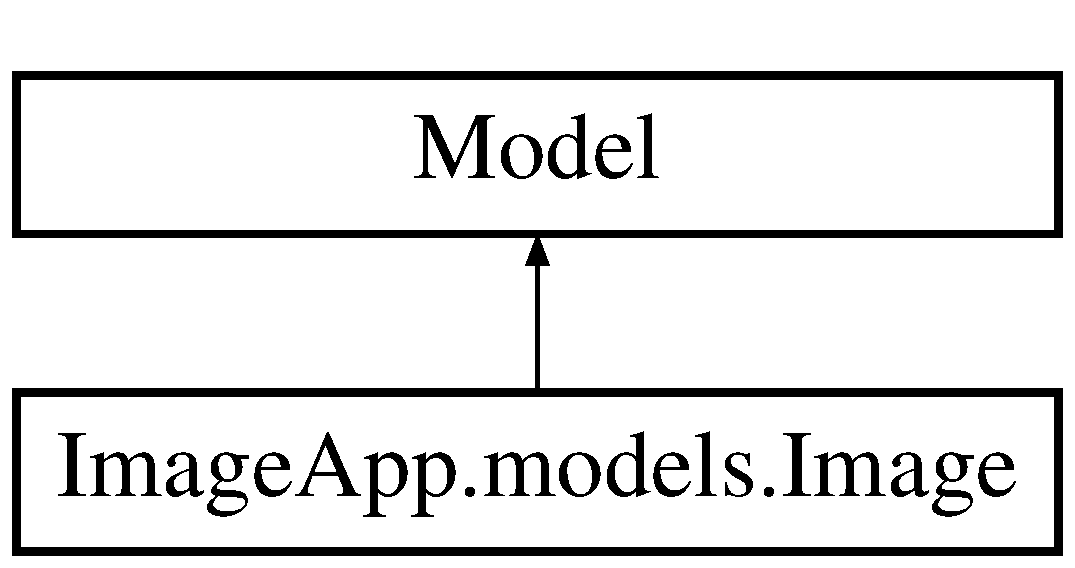
\includegraphics[height=2.000000cm]{class_image_app_1_1models_1_1_image}
\end{center}
\end{figure}
\subsection*{Static Public Attributes}
\begin{DoxyCompactItemize}
\item 
\mbox{\hyperlink{class_image_app_1_1models_1_1_image_a22b593efe01ca4fd50122621459c4d0e}{title}} = models.\+Char\+Field(max\+\_\+length=16,default=\char`\"{}Default\+Title\char`\"{})
\item 
\mbox{\hyperlink{class_image_app_1_1models_1_1_image_a03e91c21c4224a3d7219e8cdc8186aec}{description}} = models.\+Text\+Field(max\+\_\+length=255)
\item 
\mbox{\hyperlink{class_image_app_1_1models_1_1_image_a51e14dc1cb0478dd234a0ed900dd97f7}{image\+Field}} = models.\+Image\+Field(default=\textquotesingle{}defaul.\+png\textquotesingle{},blank=True)
\end{DoxyCompactItemize}


\subsection{Member Data Documentation}
\mbox{\Hypertarget{class_image_app_1_1models_1_1_image_a03e91c21c4224a3d7219e8cdc8186aec}\label{class_image_app_1_1models_1_1_image_a03e91c21c4224a3d7219e8cdc8186aec}} 
\index{Image\+App\+::models\+::\+Image@{Image\+App\+::models\+::\+Image}!description@{description}}
\index{description@{description}!Image\+App\+::models\+::\+Image@{Image\+App\+::models\+::\+Image}}
\subsubsection{\texorpdfstring{description}{description}}
{\footnotesize\ttfamily Image\+App.\+models.\+Image.\+description = models.\+Text\+Field(max\+\_\+length=255)\hspace{0.3cm}{\ttfamily [static]}}

\mbox{\Hypertarget{class_image_app_1_1models_1_1_image_a51e14dc1cb0478dd234a0ed900dd97f7}\label{class_image_app_1_1models_1_1_image_a51e14dc1cb0478dd234a0ed900dd97f7}} 
\index{Image\+App\+::models\+::\+Image@{Image\+App\+::models\+::\+Image}!image\+Field@{image\+Field}}
\index{image\+Field@{image\+Field}!Image\+App\+::models\+::\+Image@{Image\+App\+::models\+::\+Image}}
\subsubsection{\texorpdfstring{image\+Field}{imageField}}
{\footnotesize\ttfamily Image\+App.\+models.\+Image.\+image\+Field = models.\+Image\+Field(default=\textquotesingle{}defaul.\+png\textquotesingle{},blank=True)\hspace{0.3cm}{\ttfamily [static]}}

\mbox{\Hypertarget{class_image_app_1_1models_1_1_image_a22b593efe01ca4fd50122621459c4d0e}\label{class_image_app_1_1models_1_1_image_a22b593efe01ca4fd50122621459c4d0e}} 
\index{Image\+App\+::models\+::\+Image@{Image\+App\+::models\+::\+Image}!title@{title}}
\index{title@{title}!Image\+App\+::models\+::\+Image@{Image\+App\+::models\+::\+Image}}
\subsubsection{\texorpdfstring{title}{title}}
{\footnotesize\ttfamily Image\+App.\+models.\+Image.\+title = models.\+Char\+Field(max\+\_\+length=16,default=\char`\"{}Default\+Title\char`\"{})\hspace{0.3cm}{\ttfamily [static]}}



The documentation for this class was generated from the following file\+:\begin{DoxyCompactItemize}
\item 
Web\+Project/\+Cell\+Segmentation/\+Image\+App/\mbox{\hyperlink{models_8py}{models.\+py}}\end{DoxyCompactItemize}

\hypertarget{class_image_app_1_1apps_1_1_imageapp_config}{}\section{Image\+App.\+apps.\+Imageapp\+Config Class Reference}
\label{class_image_app_1_1apps_1_1_imageapp_config}\index{Image\+App.\+apps.\+Imageapp\+Config@{Image\+App.\+apps.\+Imageapp\+Config}}
Inheritance diagram for Image\+App.\+apps.\+Imageapp\+Config\+:\begin{figure}[H]
\begin{center}
\leavevmode
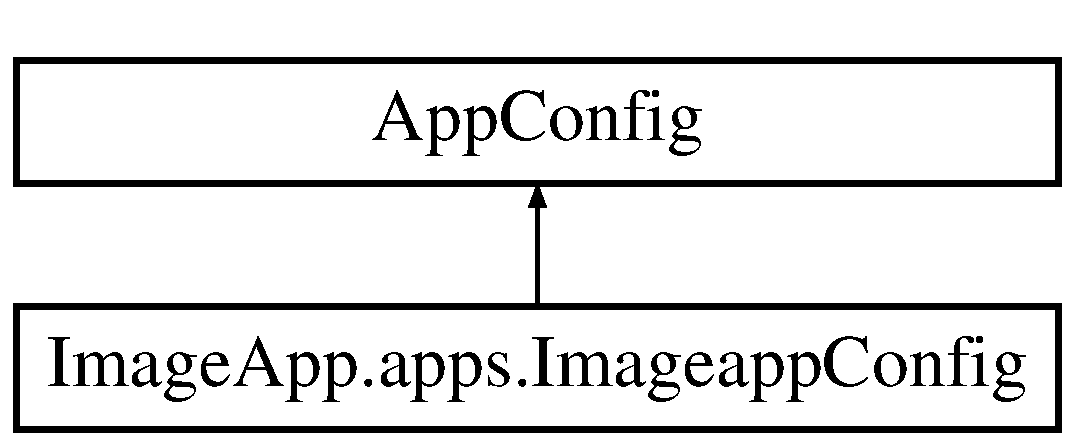
\includegraphics[height=2.000000cm]{class_image_app_1_1apps_1_1_imageapp_config}
\end{center}
\end{figure}
\subsection*{Static Public Attributes}
\begin{DoxyCompactItemize}
\item 
string \mbox{\hyperlink{class_image_app_1_1apps_1_1_imageapp_config_aee520d86c18e29442022b02d9f2646d3}{name}} = \textquotesingle{}Image\+App\textquotesingle{}
\end{DoxyCompactItemize}


\subsection{Member Data Documentation}
\mbox{\Hypertarget{class_image_app_1_1apps_1_1_imageapp_config_aee520d86c18e29442022b02d9f2646d3}\label{class_image_app_1_1apps_1_1_imageapp_config_aee520d86c18e29442022b02d9f2646d3}} 
\index{Image\+App\+::apps\+::\+Imageapp\+Config@{Image\+App\+::apps\+::\+Imageapp\+Config}!name@{name}}
\index{name@{name}!Image\+App\+::apps\+::\+Imageapp\+Config@{Image\+App\+::apps\+::\+Imageapp\+Config}}
\subsubsection{\texorpdfstring{name}{name}}
{\footnotesize\ttfamily string Image\+App.\+apps.\+Imageapp\+Config.\+name = \textquotesingle{}Image\+App\textquotesingle{}\hspace{0.3cm}{\ttfamily [static]}}



The documentation for this class was generated from the following file\+:\begin{DoxyCompactItemize}
\item 
Web\+Project/\+Cell\+Segmentation/\+Image\+App/\mbox{\hyperlink{apps_8py}{apps.\+py}}\end{DoxyCompactItemize}

\hypertarget{class_image_app_1_1forms_1_1_image_form}{}\section{Image\+App.\+forms.\+Image\+Form Class Reference}
\label{class_image_app_1_1forms_1_1_image_form}\index{Image\+App.\+forms.\+Image\+Form@{Image\+App.\+forms.\+Image\+Form}}


Formulario para la creación de una instancia de imagen.  


Inheritance diagram for Image\+App.\+forms.\+Image\+Form\+:\begin{figure}[H]
\begin{center}
\leavevmode
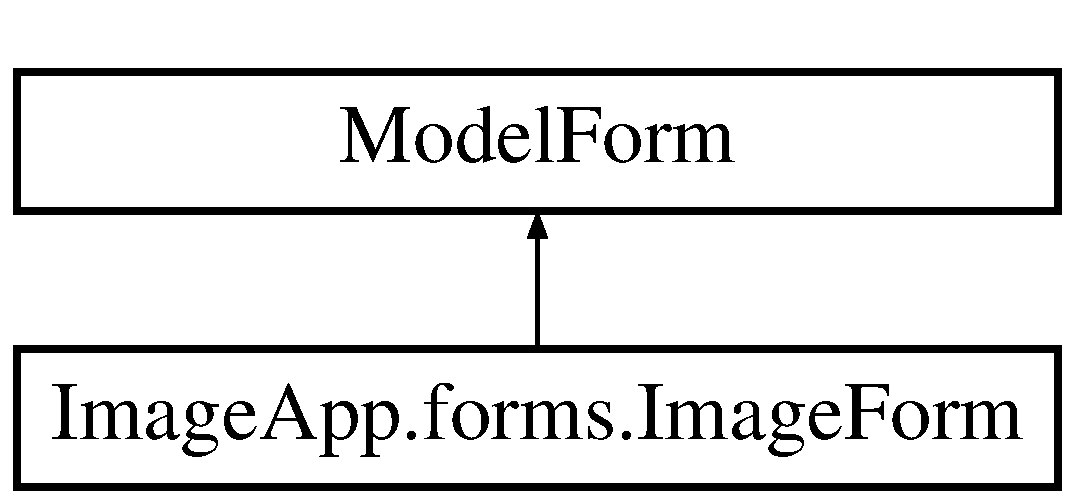
\includegraphics[height=2.000000cm]{class_image_app_1_1forms_1_1_image_form}
\end{center}
\end{figure}
\subsection*{Classes}
\begin{DoxyCompactItemize}
\item 
class \mbox{\hyperlink{class_image_app_1_1forms_1_1_image_form_1_1_meta}{Meta}}
\end{DoxyCompactItemize}


\subsection{Detailed Description}
Formulario para la creación de una instancia de imagen. 

The documentation for this class was generated from the following file\+:\begin{DoxyCompactItemize}
\item 
Web\+Project/\+Cell\+Segmentation/\+Image\+App/\mbox{\hyperlink{forms_8py}{forms.\+py}}\end{DoxyCompactItemize}

\hypertarget{class_image_app_1_1forms_1_1_image_form_1_1_meta}{}\section{Image\+App.\+forms.\+Image\+Form.\+Meta Class Reference}
\label{class_image_app_1_1forms_1_1_image_form_1_1_meta}\index{Image\+App.\+forms.\+Image\+Form.\+Meta@{Image\+App.\+forms.\+Image\+Form.\+Meta}}
\subsection*{Static Public Attributes}
\begin{DoxyCompactItemize}
\item 
\mbox{\hyperlink{class_image_app_1_1forms_1_1_image_form_1_1_meta_a6244734a872c87c5026656e8cf3f8011}{model}} = \mbox{\hyperlink{class_image_app_1_1models_1_1_image}{Image}}
\item 
list \mbox{\hyperlink{class_image_app_1_1forms_1_1_image_form_1_1_meta_a25953e0a5d7f49e62c876f6c88a0225e}{fields}}
\end{DoxyCompactItemize}


\subsection{Member Data Documentation}
\mbox{\Hypertarget{class_image_app_1_1forms_1_1_image_form_1_1_meta_a25953e0a5d7f49e62c876f6c88a0225e}\label{class_image_app_1_1forms_1_1_image_form_1_1_meta_a25953e0a5d7f49e62c876f6c88a0225e}} 
\index{Image\+App\+::forms\+::\+Image\+Form\+::\+Meta@{Image\+App\+::forms\+::\+Image\+Form\+::\+Meta}!fields@{fields}}
\index{fields@{fields}!Image\+App\+::forms\+::\+Image\+Form\+::\+Meta@{Image\+App\+::forms\+::\+Image\+Form\+::\+Meta}}
\subsubsection{\texorpdfstring{fields}{fields}}
{\footnotesize\ttfamily list Image\+App.\+forms.\+Image\+Form.\+Meta.\+fields\hspace{0.3cm}{\ttfamily [static]}}

{\bfseries Initial value\+:}
\begin{DoxyCode}
=  [
            \textcolor{stringliteral}{'title'},
            \textcolor{stringliteral}{'description'},
            \textcolor{stringliteral}{'imageField'}
        ]
\end{DoxyCode}
\mbox{\Hypertarget{class_image_app_1_1forms_1_1_image_form_1_1_meta_a6244734a872c87c5026656e8cf3f8011}\label{class_image_app_1_1forms_1_1_image_form_1_1_meta_a6244734a872c87c5026656e8cf3f8011}} 
\index{Image\+App\+::forms\+::\+Image\+Form\+::\+Meta@{Image\+App\+::forms\+::\+Image\+Form\+::\+Meta}!model@{model}}
\index{model@{model}!Image\+App\+::forms\+::\+Image\+Form\+::\+Meta@{Image\+App\+::forms\+::\+Image\+Form\+::\+Meta}}
\subsubsection{\texorpdfstring{model}{model}}
{\footnotesize\ttfamily Image\+App.\+forms.\+Image\+Form.\+Meta.\+model = \mbox{\hyperlink{class_image_app_1_1models_1_1_image}{Image}}\hspace{0.3cm}{\ttfamily [static]}}



The documentation for this class was generated from the following file\+:\begin{DoxyCompactItemize}
\item 
Web\+Project/\+Cell\+Segmentation/\+Image\+App/\mbox{\hyperlink{forms_8py}{forms.\+py}}\end{DoxyCompactItemize}

\hypertarget{class_image_app_1_1migrations_1_10004__auto__20180819__1722_1_1_migration}{}\section{Image\+App.\+migrations.0004\+\_\+auto\+\_\+20180819\+\_\+1722.Migration Class Reference}
\label{class_image_app_1_1migrations_1_10004__auto__20180819__1722_1_1_migration}\index{Image\+App.\+migrations.\+0004\+\_\+auto\+\_\+20180819\+\_\+1722.\+Migration@{Image\+App.\+migrations.\+0004\+\_\+auto\+\_\+20180819\+\_\+1722.\+Migration}}
Inheritance diagram for Image\+App.\+migrations.0004\+\_\+auto\+\_\+20180819\+\_\+1722.Migration\+:\begin{figure}[H]
\begin{center}
\leavevmode
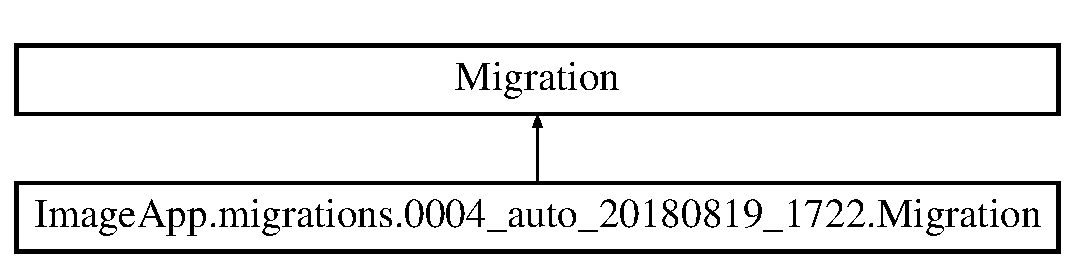
\includegraphics[height=2.000000cm]{class_image_app_1_1migrations_1_10004__auto__20180819__1722_1_1_migration}
\end{center}
\end{figure}
\subsection*{Static Public Attributes}
\begin{DoxyCompactItemize}
\item 
list \mbox{\hyperlink{class_image_app_1_1migrations_1_10004__auto__20180819__1722_1_1_migration_ac162d538fef083d35dca6ff268b2dfb0}{dependencies}}
\item 
list \mbox{\hyperlink{class_image_app_1_1migrations_1_10004__auto__20180819__1722_1_1_migration_ab2af20850457c5864ba5ea409e91d9e1}{operations}}
\end{DoxyCompactItemize}


\subsection{Member Data Documentation}
\mbox{\Hypertarget{class_image_app_1_1migrations_1_10004__auto__20180819__1722_1_1_migration_ac162d538fef083d35dca6ff268b2dfb0}\label{class_image_app_1_1migrations_1_10004__auto__20180819__1722_1_1_migration_ac162d538fef083d35dca6ff268b2dfb0}} 
\index{Image\+App\+::migrations\+::0004\+\_\+auto\+\_\+20180819\+\_\+1722\+::\+Migration@{Image\+App\+::migrations\+::0004\+\_\+auto\+\_\+20180819\+\_\+1722\+::\+Migration}!dependencies@{dependencies}}
\index{dependencies@{dependencies}!Image\+App\+::migrations\+::0004\+\_\+auto\+\_\+20180819\+\_\+1722\+::\+Migration@{Image\+App\+::migrations\+::0004\+\_\+auto\+\_\+20180819\+\_\+1722\+::\+Migration}}
\subsubsection{\texorpdfstring{dependencies}{dependencies}}
{\footnotesize\ttfamily list Image\+App.\+migrations.\+0004\+\_\+auto\+\_\+20180819\+\_\+1722.\+Migration.\+dependencies\hspace{0.3cm}{\ttfamily [static]}}

{\bfseries Initial value\+:}
\begin{DoxyCode}
=  [
        (\textcolor{stringliteral}{'ImageApp'}, \textcolor{stringliteral}{'0003\_auto\_20180818\_1425'}),
    ]
\end{DoxyCode}
\mbox{\Hypertarget{class_image_app_1_1migrations_1_10004__auto__20180819__1722_1_1_migration_ab2af20850457c5864ba5ea409e91d9e1}\label{class_image_app_1_1migrations_1_10004__auto__20180819__1722_1_1_migration_ab2af20850457c5864ba5ea409e91d9e1}} 
\index{Image\+App\+::migrations\+::0004\+\_\+auto\+\_\+20180819\+\_\+1722\+::\+Migration@{Image\+App\+::migrations\+::0004\+\_\+auto\+\_\+20180819\+\_\+1722\+::\+Migration}!operations@{operations}}
\index{operations@{operations}!Image\+App\+::migrations\+::0004\+\_\+auto\+\_\+20180819\+\_\+1722\+::\+Migration@{Image\+App\+::migrations\+::0004\+\_\+auto\+\_\+20180819\+\_\+1722\+::\+Migration}}
\subsubsection{\texorpdfstring{operations}{operations}}
{\footnotesize\ttfamily list Image\+App.\+migrations.\+0004\+\_\+auto\+\_\+20180819\+\_\+1722.\+Migration.\+operations\hspace{0.3cm}{\ttfamily [static]}}

{\bfseries Initial value\+:}
\begin{DoxyCode}
=  [
        migrations.AlterField(
            model\_name=\textcolor{stringliteral}{'image'},
            name=\textcolor{stringliteral}{'description'},
            field=models.TextField(max\_length=255),
        ),
        migrations.AlterField(
            model\_name=\textcolor{stringliteral}{'image'},
            name=\textcolor{stringliteral}{'title'},
            field=models.CharField(default=\textcolor{stringliteral}{'DefaultTitle'}, max\_length=16),
        ),
    ]
\end{DoxyCode}


The documentation for this class was generated from the following file\+:\begin{DoxyCompactItemize}
\item 
Web\+Project/\+Cell\+Segmentation/\+Image\+App/migrations/\mbox{\hyperlink{0004__auto__20180819__1722_8py}{0004\+\_\+auto\+\_\+20180819\+\_\+1722.\+py}}\end{DoxyCompactItemize}

\hypertarget{class_image_app_1_1migrations_1_10001__initial_1_1_migration}{}\section{Image\+App.\+migrations.0001\+\_\+initial.Migration Class Reference}
\label{class_image_app_1_1migrations_1_10001__initial_1_1_migration}\index{Image\+App.\+migrations.\+0001\+\_\+initial.\+Migration@{Image\+App.\+migrations.\+0001\+\_\+initial.\+Migration}}
Inheritance diagram for Image\+App.\+migrations.0001\+\_\+initial.Migration\+:\begin{figure}[H]
\begin{center}
\leavevmode
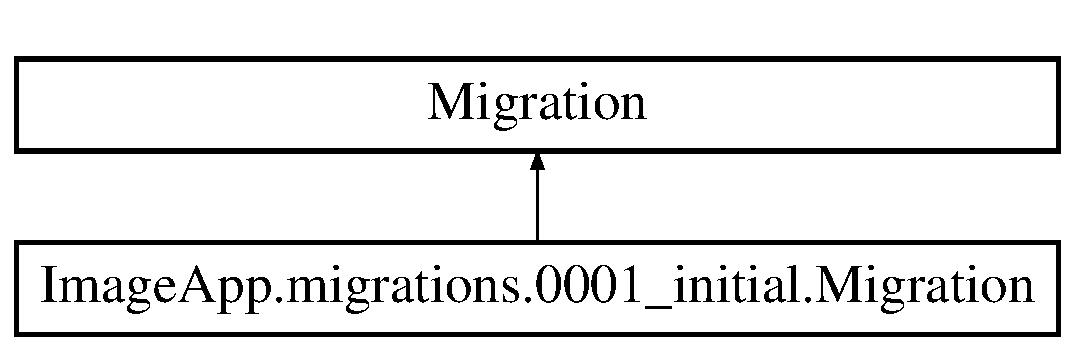
\includegraphics[height=2.000000cm]{class_image_app_1_1migrations_1_10001__initial_1_1_migration}
\end{center}
\end{figure}
\subsection*{Static Public Attributes}
\begin{DoxyCompactItemize}
\item 
bool \mbox{\hyperlink{class_image_app_1_1migrations_1_10001__initial_1_1_migration_ab7c1550e482a827afc880d61aef3d582}{initial}} = True
\item 
list \mbox{\hyperlink{class_image_app_1_1migrations_1_10001__initial_1_1_migration_a0948ef2c2b5eecf68e435d8cf3891757}{dependencies}}
\item 
list \mbox{\hyperlink{class_image_app_1_1migrations_1_10001__initial_1_1_migration_a3e24a94fd90e7788a2bddffc7a529b16}{operations}}
\end{DoxyCompactItemize}


\subsection{Member Data Documentation}
\mbox{\Hypertarget{class_image_app_1_1migrations_1_10001__initial_1_1_migration_a0948ef2c2b5eecf68e435d8cf3891757}\label{class_image_app_1_1migrations_1_10001__initial_1_1_migration_a0948ef2c2b5eecf68e435d8cf3891757}} 
\index{Image\+App\+::migrations\+::0001\+\_\+initial\+::\+Migration@{Image\+App\+::migrations\+::0001\+\_\+initial\+::\+Migration}!dependencies@{dependencies}}
\index{dependencies@{dependencies}!Image\+App\+::migrations\+::0001\+\_\+initial\+::\+Migration@{Image\+App\+::migrations\+::0001\+\_\+initial\+::\+Migration}}
\subsubsection{\texorpdfstring{dependencies}{dependencies}}
{\footnotesize\ttfamily list Image\+App.\+migrations.\+0001\+\_\+initial.\+Migration.\+dependencies\hspace{0.3cm}{\ttfamily [static]}}

{\bfseries Initial value\+:}
\begin{DoxyCode}
=  [
    ]
\end{DoxyCode}
\mbox{\Hypertarget{class_image_app_1_1migrations_1_10001__initial_1_1_migration_ab7c1550e482a827afc880d61aef3d582}\label{class_image_app_1_1migrations_1_10001__initial_1_1_migration_ab7c1550e482a827afc880d61aef3d582}} 
\index{Image\+App\+::migrations\+::0001\+\_\+initial\+::\+Migration@{Image\+App\+::migrations\+::0001\+\_\+initial\+::\+Migration}!initial@{initial}}
\index{initial@{initial}!Image\+App\+::migrations\+::0001\+\_\+initial\+::\+Migration@{Image\+App\+::migrations\+::0001\+\_\+initial\+::\+Migration}}
\subsubsection{\texorpdfstring{initial}{initial}}
{\footnotesize\ttfamily bool Image\+App.\+migrations.\+0001\+\_\+initial.\+Migration.\+initial = True\hspace{0.3cm}{\ttfamily [static]}}

\mbox{\Hypertarget{class_image_app_1_1migrations_1_10001__initial_1_1_migration_a3e24a94fd90e7788a2bddffc7a529b16}\label{class_image_app_1_1migrations_1_10001__initial_1_1_migration_a3e24a94fd90e7788a2bddffc7a529b16}} 
\index{Image\+App\+::migrations\+::0001\+\_\+initial\+::\+Migration@{Image\+App\+::migrations\+::0001\+\_\+initial\+::\+Migration}!operations@{operations}}
\index{operations@{operations}!Image\+App\+::migrations\+::0001\+\_\+initial\+::\+Migration@{Image\+App\+::migrations\+::0001\+\_\+initial\+::\+Migration}}
\subsubsection{\texorpdfstring{operations}{operations}}
{\footnotesize\ttfamily list Image\+App.\+migrations.\+0001\+\_\+initial.\+Migration.\+operations\hspace{0.3cm}{\ttfamily [static]}}

{\bfseries Initial value\+:}
\begin{DoxyCode}
=  [
        migrations.CreateModel(
            name=\textcolor{stringliteral}{'Image'},
            fields=[
                (\textcolor{stringliteral}{'id'}, models.AutoField(auto\_created=\textcolor{keyword}{True}, primary\_key=\textcolor{keyword}{True}, serialize=\textcolor{keyword}{False}, verbose\_name=\textcolor{stringliteral}{
      'ID'})),
                (\textcolor{stringliteral}{'title'}, models.TextField()),
                (\textcolor{stringliteral}{'description'}, models.TextField()),
            ],
        ),
    ]
\end{DoxyCode}


The documentation for this class was generated from the following file\+:\begin{DoxyCompactItemize}
\item 
Web\+Project/\+Cell\+Segmentation/\+Image\+App/migrations/\mbox{\hyperlink{0001__initial_8py}{0001\+\_\+initial.\+py}}\end{DoxyCompactItemize}

\hypertarget{class_image_app_1_1migrations_1_10003__auto__20180818__1425_1_1_migration}{}\section{Image\+App.\+migrations.0003\+\_\+auto\+\_\+20180818\+\_\+1425.Migration Class Reference}
\label{class_image_app_1_1migrations_1_10003__auto__20180818__1425_1_1_migration}\index{Image\+App.\+migrations.\+0003\+\_\+auto\+\_\+20180818\+\_\+1425.\+Migration@{Image\+App.\+migrations.\+0003\+\_\+auto\+\_\+20180818\+\_\+1425.\+Migration}}
Inheritance diagram for Image\+App.\+migrations.0003\+\_\+auto\+\_\+20180818\+\_\+1425.Migration\+:\begin{figure}[H]
\begin{center}
\leavevmode
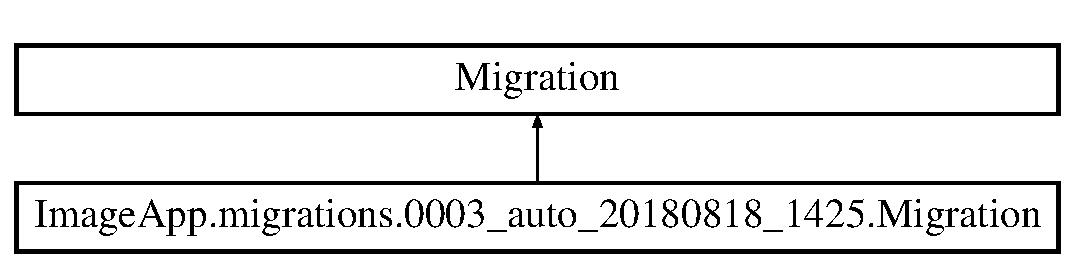
\includegraphics[height=2.000000cm]{class_image_app_1_1migrations_1_10003__auto__20180818__1425_1_1_migration}
\end{center}
\end{figure}
\subsection*{Static Public Attributes}
\begin{DoxyCompactItemize}
\item 
list \mbox{\hyperlink{class_image_app_1_1migrations_1_10003__auto__20180818__1425_1_1_migration_a33c13fdbeb1e5e28d03d1a1fc391dad3}{dependencies}}
\item 
list \mbox{\hyperlink{class_image_app_1_1migrations_1_10003__auto__20180818__1425_1_1_migration_aae609b480f1a2542bd52396572fc1574}{operations}}
\end{DoxyCompactItemize}


\subsection{Member Data Documentation}
\mbox{\Hypertarget{class_image_app_1_1migrations_1_10003__auto__20180818__1425_1_1_migration_a33c13fdbeb1e5e28d03d1a1fc391dad3}\label{class_image_app_1_1migrations_1_10003__auto__20180818__1425_1_1_migration_a33c13fdbeb1e5e28d03d1a1fc391dad3}} 
\index{Image\+App\+::migrations\+::0003\+\_\+auto\+\_\+20180818\+\_\+1425\+::\+Migration@{Image\+App\+::migrations\+::0003\+\_\+auto\+\_\+20180818\+\_\+1425\+::\+Migration}!dependencies@{dependencies}}
\index{dependencies@{dependencies}!Image\+App\+::migrations\+::0003\+\_\+auto\+\_\+20180818\+\_\+1425\+::\+Migration@{Image\+App\+::migrations\+::0003\+\_\+auto\+\_\+20180818\+\_\+1425\+::\+Migration}}
\subsubsection{\texorpdfstring{dependencies}{dependencies}}
{\footnotesize\ttfamily list Image\+App.\+migrations.\+0003\+\_\+auto\+\_\+20180818\+\_\+1425.\+Migration.\+dependencies\hspace{0.3cm}{\ttfamily [static]}}

{\bfseries Initial value\+:}
\begin{DoxyCode}
=  [
        (\textcolor{stringliteral}{'ImageApp'}, \textcolor{stringliteral}{'0002\_image\_imagefile'}),
    ]
\end{DoxyCode}
\mbox{\Hypertarget{class_image_app_1_1migrations_1_10003__auto__20180818__1425_1_1_migration_aae609b480f1a2542bd52396572fc1574}\label{class_image_app_1_1migrations_1_10003__auto__20180818__1425_1_1_migration_aae609b480f1a2542bd52396572fc1574}} 
\index{Image\+App\+::migrations\+::0003\+\_\+auto\+\_\+20180818\+\_\+1425\+::\+Migration@{Image\+App\+::migrations\+::0003\+\_\+auto\+\_\+20180818\+\_\+1425\+::\+Migration}!operations@{operations}}
\index{operations@{operations}!Image\+App\+::migrations\+::0003\+\_\+auto\+\_\+20180818\+\_\+1425\+::\+Migration@{Image\+App\+::migrations\+::0003\+\_\+auto\+\_\+20180818\+\_\+1425\+::\+Migration}}
\subsubsection{\texorpdfstring{operations}{operations}}
{\footnotesize\ttfamily list Image\+App.\+migrations.\+0003\+\_\+auto\+\_\+20180818\+\_\+1425.\+Migration.\+operations\hspace{0.3cm}{\ttfamily [static]}}

{\bfseries Initial value\+:}
\begin{DoxyCode}
=  [
        migrations.RenameField(
            model\_name=\textcolor{stringliteral}{'image'},
            old\_name=\textcolor{stringliteral}{'imageFile'},
            new\_name=\textcolor{stringliteral}{'imageField'},
        ),
    ]
\end{DoxyCode}


The documentation for this class was generated from the following file\+:\begin{DoxyCompactItemize}
\item 
Web\+Project/\+Cell\+Segmentation/\+Image\+App/migrations/\mbox{\hyperlink{0003__auto__20180818__1425_8py}{0003\+\_\+auto\+\_\+20180818\+\_\+1425.\+py}}\end{DoxyCompactItemize}

\hypertarget{class_image_app_1_1migrations_1_10002__image__imagefile_1_1_migration}{}\section{Image\+App.\+migrations.0002\+\_\+image\+\_\+imagefile.Migration Class Reference}
\label{class_image_app_1_1migrations_1_10002__image__imagefile_1_1_migration}\index{Image\+App.\+migrations.\+0002\+\_\+image\+\_\+imagefile.\+Migration@{Image\+App.\+migrations.\+0002\+\_\+image\+\_\+imagefile.\+Migration}}
Inheritance diagram for Image\+App.\+migrations.0002\+\_\+image\+\_\+imagefile.Migration\+:\begin{figure}[H]
\begin{center}
\leavevmode
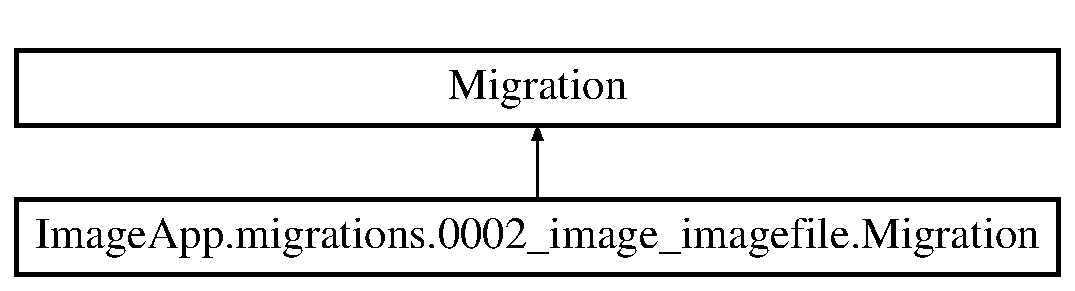
\includegraphics[height=2.000000cm]{class_image_app_1_1migrations_1_10002__image__imagefile_1_1_migration}
\end{center}
\end{figure}
\subsection*{Static Public Attributes}
\begin{DoxyCompactItemize}
\item 
list \mbox{\hyperlink{class_image_app_1_1migrations_1_10002__image__imagefile_1_1_migration_ada6489c4f14dcd26514c8a713be7bd19}{dependencies}}
\item 
list \mbox{\hyperlink{class_image_app_1_1migrations_1_10002__image__imagefile_1_1_migration_a69c49e7f79f172c63206a38fb765d519}{operations}}
\end{DoxyCompactItemize}


\subsection{Member Data Documentation}
\mbox{\Hypertarget{class_image_app_1_1migrations_1_10002__image__imagefile_1_1_migration_ada6489c4f14dcd26514c8a713be7bd19}\label{class_image_app_1_1migrations_1_10002__image__imagefile_1_1_migration_ada6489c4f14dcd26514c8a713be7bd19}} 
\index{Image\+App\+::migrations\+::0002\+\_\+image\+\_\+imagefile\+::\+Migration@{Image\+App\+::migrations\+::0002\+\_\+image\+\_\+imagefile\+::\+Migration}!dependencies@{dependencies}}
\index{dependencies@{dependencies}!Image\+App\+::migrations\+::0002\+\_\+image\+\_\+imagefile\+::\+Migration@{Image\+App\+::migrations\+::0002\+\_\+image\+\_\+imagefile\+::\+Migration}}
\subsubsection{\texorpdfstring{dependencies}{dependencies}}
{\footnotesize\ttfamily list Image\+App.\+migrations.\+0002\+\_\+image\+\_\+imagefile.\+Migration.\+dependencies\hspace{0.3cm}{\ttfamily [static]}}

{\bfseries Initial value\+:}
\begin{DoxyCode}
=  [
        (\textcolor{stringliteral}{'ImageApp'}, \textcolor{stringliteral}{'0001\_initial'}),
    ]
\end{DoxyCode}
\mbox{\Hypertarget{class_image_app_1_1migrations_1_10002__image__imagefile_1_1_migration_a69c49e7f79f172c63206a38fb765d519}\label{class_image_app_1_1migrations_1_10002__image__imagefile_1_1_migration_a69c49e7f79f172c63206a38fb765d519}} 
\index{Image\+App\+::migrations\+::0002\+\_\+image\+\_\+imagefile\+::\+Migration@{Image\+App\+::migrations\+::0002\+\_\+image\+\_\+imagefile\+::\+Migration}!operations@{operations}}
\index{operations@{operations}!Image\+App\+::migrations\+::0002\+\_\+image\+\_\+imagefile\+::\+Migration@{Image\+App\+::migrations\+::0002\+\_\+image\+\_\+imagefile\+::\+Migration}}
\subsubsection{\texorpdfstring{operations}{operations}}
{\footnotesize\ttfamily list Image\+App.\+migrations.\+0002\+\_\+image\+\_\+imagefile.\+Migration.\+operations\hspace{0.3cm}{\ttfamily [static]}}

{\bfseries Initial value\+:}
\begin{DoxyCode}
=  [
        migrations.AddField(
            model\_name=\textcolor{stringliteral}{'image'},
            name=\textcolor{stringliteral}{'imageFile'},
            field=models.ImageField(blank=\textcolor{keyword}{True}, default=\textcolor{stringliteral}{'defaul.png'}, upload\_to=\textcolor{stringliteral}{''}),
        ),
    ]
\end{DoxyCode}


The documentation for this class was generated from the following file\+:\begin{DoxyCompactItemize}
\item 
Web\+Project/\+Cell\+Segmentation/\+Image\+App/migrations/\mbox{\hyperlink{0002__image__imagefile_8py}{0002\+\_\+image\+\_\+imagefile.\+py}}\end{DoxyCompactItemize}

\hypertarget{class_kera_q_a_1_1_test_keras}{}\section{Kera\+Q\+A.\+Test\+Keras Class Reference}
\label{class_kera_q_a_1_1_test_keras}\index{Kera\+Q\+A.\+Test\+Keras@{Kera\+Q\+A.\+Test\+Keras}}
Inheritance diagram for Kera\+Q\+A.\+Test\+Keras\+:\begin{figure}[H]
\begin{center}
\leavevmode
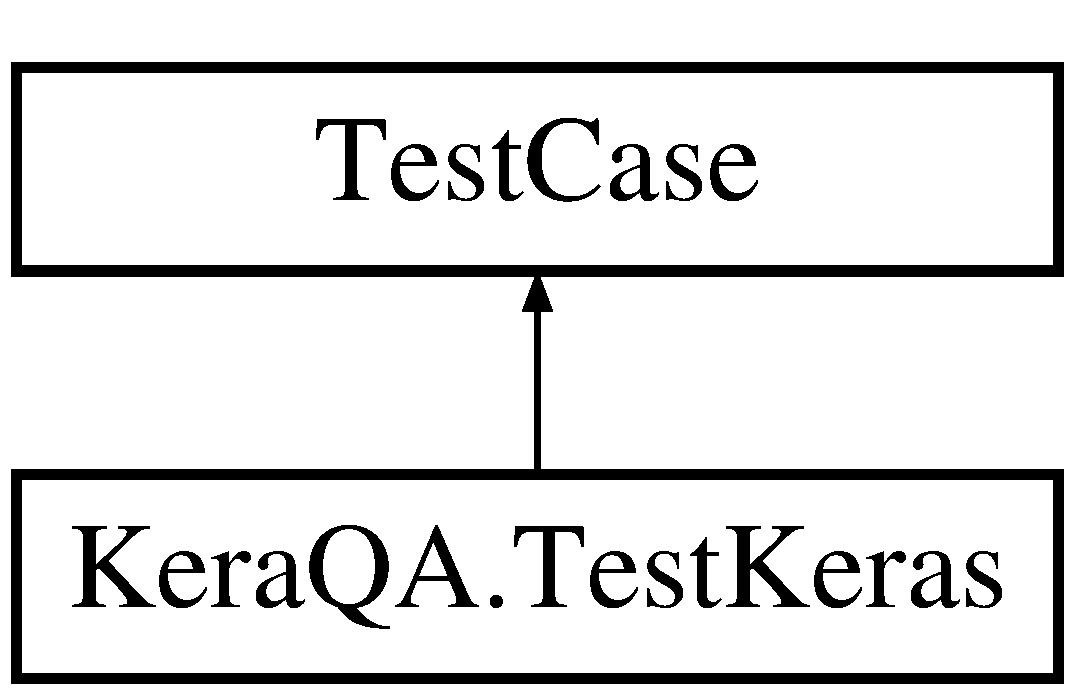
\includegraphics[height=2.000000cm]{class_kera_q_a_1_1_test_keras}
\end{center}
\end{figure}
\subsection*{Public Member Functions}
\begin{DoxyCompactItemize}
\item 
def \mbox{\hyperlink{class_kera_q_a_1_1_test_keras_a8861b428188d639538a61d0b20fede22}{test\+\_\+carga\+\_\+modelo}} (self)
\item 
def \mbox{\hyperlink{class_kera_q_a_1_1_test_keras_aa9ec17e7cad0fab158b9686266f80ec6}{test\+\_\+compilacion\+\_\+modelo}} (self)
\end{DoxyCompactItemize}


\subsection{Member Function Documentation}
\mbox{\Hypertarget{class_kera_q_a_1_1_test_keras_a8861b428188d639538a61d0b20fede22}\label{class_kera_q_a_1_1_test_keras_a8861b428188d639538a61d0b20fede22}} 
\index{Kera\+Q\+A\+::\+Test\+Keras@{Kera\+Q\+A\+::\+Test\+Keras}!test\+\_\+carga\+\_\+modelo@{test\+\_\+carga\+\_\+modelo}}
\index{test\+\_\+carga\+\_\+modelo@{test\+\_\+carga\+\_\+modelo}!Kera\+Q\+A\+::\+Test\+Keras@{Kera\+Q\+A\+::\+Test\+Keras}}
\subsubsection{\texorpdfstring{test\+\_\+carga\+\_\+modelo()}{test\_carga\_modelo()}}
{\footnotesize\ttfamily def Kera\+Q\+A.\+Test\+Keras.\+test\+\_\+carga\+\_\+modelo (\begin{DoxyParamCaption}\item[{}]{self }\end{DoxyParamCaption})}

\mbox{\Hypertarget{class_kera_q_a_1_1_test_keras_aa9ec17e7cad0fab158b9686266f80ec6}\label{class_kera_q_a_1_1_test_keras_aa9ec17e7cad0fab158b9686266f80ec6}} 
\index{Kera\+Q\+A\+::\+Test\+Keras@{Kera\+Q\+A\+::\+Test\+Keras}!test\+\_\+compilacion\+\_\+modelo@{test\+\_\+compilacion\+\_\+modelo}}
\index{test\+\_\+compilacion\+\_\+modelo@{test\+\_\+compilacion\+\_\+modelo}!Kera\+Q\+A\+::\+Test\+Keras@{Kera\+Q\+A\+::\+Test\+Keras}}
\subsubsection{\texorpdfstring{test\+\_\+compilacion\+\_\+modelo()}{test\_compilacion\_modelo()}}
{\footnotesize\ttfamily def Kera\+Q\+A.\+Test\+Keras.\+test\+\_\+compilacion\+\_\+modelo (\begin{DoxyParamCaption}\item[{}]{self }\end{DoxyParamCaption})}



The documentation for this class was generated from the following file\+:\begin{DoxyCompactItemize}
\item 
keras\+Segmentation/\mbox{\hyperlink{_kera_q_a_8py}{Kera\+Q\+A.\+py}}\end{DoxyCompactItemize}

\chapter{File Documentation}
\hypertarget{_kera_q_a_8py}{}\section{keras\+Segmentation/\+Kera\+QA.py File Reference}
\label{_kera_q_a_8py}\index{keras\+Segmentation/\+Kera\+Q\+A.\+py@{keras\+Segmentation/\+Kera\+Q\+A.\+py}}
\subsection*{Classes}
\begin{DoxyCompactItemize}
\item 
class \mbox{\hyperlink{class_kera_q_a_1_1_test_keras}{Kera\+Q\+A.\+Test\+Keras}}
\end{DoxyCompactItemize}
\subsection*{Namespaces}
\begin{DoxyCompactItemize}
\item 
 \mbox{\hyperlink{namespace_kera_q_a}{Kera\+QA}}
\end{DoxyCompactItemize}

\hypertarget{modelo_8py}{}\section{keras\+Segmentation/modelo.py File Reference}
\label{modelo_8py}\index{keras\+Segmentation/modelo.\+py@{keras\+Segmentation/modelo.\+py}}
\subsection*{Namespaces}
\begin{DoxyCompactItemize}
\item 
 \mbox{\hyperlink{namespacemodelo}{modelo}}
\end{DoxyCompactItemize}
\subsection*{Functions}
\begin{DoxyCompactItemize}
\item 
def \mbox{\hyperlink{namespacemodelo_a1003684c17149ab9b5f89f9e77b687a7}{modelo.\+cargar\+\_\+modelo}} (nombre\+\_\+modelo)
\begin{DoxyCompactList}\small\item\em Carga un modelo previamente generado por keras, con formato .h5. \end{DoxyCompactList}\item 
def \mbox{\hyperlink{namespacemodelo_a4a48c138f410a4c8a4021e2696b7d5c6}{modelo.\+compiler\+\_\+modelo}} (modelo)
\begin{DoxyCompactList}\small\item\em Compila un modelo previamente cargado para luego ser ejecutado. \end{DoxyCompactList}\end{DoxyCompactItemize}

\hypertarget{manejo_archivos_c_s_v_8py}{}\section{pandas/manejo\+Archivos\+C\+SV.py File Reference}
\label{manejo_archivos_c_s_v_8py}\index{pandas/manejo\+Archivos\+C\+S\+V.\+py@{pandas/manejo\+Archivos\+C\+S\+V.\+py}}
\subsection*{Namespaces}
\begin{DoxyCompactItemize}
\item 
 \mbox{\hyperlink{namespacemanejo_archivos_c_s_v}{manejo\+Archivos\+C\+SV}}
\end{DoxyCompactItemize}
\subsection*{Functions}
\begin{DoxyCompactItemize}
\item 
def \mbox{\hyperlink{namespacemanejo_archivos_c_s_v_af84ef6e5a0591162a0b781c11145845e}{manejo\+Archivos\+C\+S\+V.\+leer\+Archivo\+C\+SV}} (nombre\+Archivo)
\begin{DoxyCompactList}\small\item\em Abre y lee un archivo de tipo C\+SV. \end{DoxyCompactList}\item 
def \mbox{\hyperlink{namespacemanejo_archivos_c_s_v_a0c9d188d26bb6dea35ce440f32015b01}{manejo\+Archivos\+C\+S\+V.\+generar\+Archivo\+C\+SV}} (nombre\+Archivo, datos)
\begin{DoxyCompactList}\small\item\em Genera un nuevo archivo tipo C\+SV. \end{DoxyCompactList}\end{DoxyCompactItemize}

\hypertarget{_cell_segmentation_2____init_____8py}{}\section{Web\+Project/\+Cell\+Segmentation/\+Cell\+Segmentation/\+\_\+\+\_\+init\+\_\+\+\_\+.py File Reference}
\label{_cell_segmentation_2____init_____8py}\index{Web\+Project/\+Cell\+Segmentation/\+Cell\+Segmentation/\+\_\+\+\_\+init\+\_\+\+\_\+.\+py@{Web\+Project/\+Cell\+Segmentation/\+Cell\+Segmentation/\+\_\+\+\_\+init\+\_\+\+\_\+.\+py}}
\subsection*{Namespaces}
\begin{DoxyCompactItemize}
\item 
 \mbox{\hyperlink{namespace_cell_segmentation}{Cell\+Segmentation}}
\end{DoxyCompactItemize}

\hypertarget{_image_app_2____init_____8py}{}\section{Web\+Project/\+Cell\+Segmentation/\+Image\+App/\+\_\+\+\_\+init\+\_\+\+\_\+.py File Reference}
\label{_image_app_2____init_____8py}\index{Web\+Project/\+Cell\+Segmentation/\+Image\+App/\+\_\+\+\_\+init\+\_\+\+\_\+.\+py@{Web\+Project/\+Cell\+Segmentation/\+Image\+App/\+\_\+\+\_\+init\+\_\+\+\_\+.\+py}}
\subsection*{Namespaces}
\begin{DoxyCompactItemize}
\item 
 \mbox{\hyperlink{namespace_image_app}{Image\+App}}
\end{DoxyCompactItemize}

\hypertarget{_image_app_2migrations_2____init_____8py}{}\section{Web\+Project/\+Cell\+Segmentation/\+Image\+App/migrations/\+\_\+\+\_\+init\+\_\+\+\_\+.py File Reference}
\label{_image_app_2migrations_2____init_____8py}\index{Web\+Project/\+Cell\+Segmentation/\+Image\+App/migrations/\+\_\+\+\_\+init\+\_\+\+\_\+.\+py@{Web\+Project/\+Cell\+Segmentation/\+Image\+App/migrations/\+\_\+\+\_\+init\+\_\+\+\_\+.\+py}}
\subsection*{Namespaces}
\begin{DoxyCompactItemize}
\item 
 \mbox{\hyperlink{namespace_image_app_1_1migrations}{Image\+App.\+migrations}}
\end{DoxyCompactItemize}

\hypertarget{settings_8py}{}\section{Web\+Project/\+Cell\+Segmentation/\+Cell\+Segmentation/settings.py File Reference}
\label{settings_8py}\index{Web\+Project/\+Cell\+Segmentation/\+Cell\+Segmentation/settings.\+py@{Web\+Project/\+Cell\+Segmentation/\+Cell\+Segmentation/settings.\+py}}
\subsection*{Namespaces}
\begin{DoxyCompactItemize}
\item 
 \mbox{\hyperlink{namespace_cell_segmentation_1_1settings}{Cell\+Segmentation.\+settings}}
\end{DoxyCompactItemize}
\subsection*{Variables}
\begin{DoxyCompactItemize}
\item 
\mbox{\hyperlink{namespace_cell_segmentation_1_1settings_a354c3e9bde5b55650a0e821028acf8c2}{Cell\+Segmentation.\+settings.\+B\+A\+S\+E\+\_\+\+D\+IR}} = os.\+path.\+dirname(os.\+path.\+dirname(os.\+path.\+abspath(\+\_\+\+\_\+file\+\_\+\+\_\+)))
\item 
string \mbox{\hyperlink{namespace_cell_segmentation_1_1settings_a2b895f9bfae7ccf648a88cc8c31c9be0}{Cell\+Segmentation.\+settings.\+S\+E\+C\+R\+E\+T\+\_\+\+K\+EY}} = \textquotesingle{}0=\$\#9\$jb$^\wedge$b0w0gf!l5+ub\#ofjd3)+jjw$^\wedge$08\#1bi9$\ast$iwqur-\/a\$=\textquotesingle{}
\item 
bool \mbox{\hyperlink{namespace_cell_segmentation_1_1settings_a787047027345638dd2b9ff2df7c1dac6}{Cell\+Segmentation.\+settings.\+D\+E\+B\+UG}} = True
\item 
list \mbox{\hyperlink{namespace_cell_segmentation_1_1settings_aa1860414aa297264b68c5d9de3c0bb3e}{Cell\+Segmentation.\+settings.\+A\+L\+L\+O\+W\+E\+D\+\_\+\+H\+O\+S\+TS}} = \mbox{[}$\,$\mbox{]}
\item 
list \mbox{\hyperlink{namespace_cell_segmentation_1_1settings_a3724321f33b3f6dd16253ddddffa7d9e}{Cell\+Segmentation.\+settings.\+I\+N\+S\+T\+A\+L\+L\+E\+D\+\_\+\+A\+P\+PS}}
\item 
list \mbox{\hyperlink{namespace_cell_segmentation_1_1settings_a9d3647228b19e6473eb9573388ea2c04}{Cell\+Segmentation.\+settings.\+M\+I\+D\+D\+L\+E\+W\+A\+RE}}
\item 
string \mbox{\hyperlink{namespace_cell_segmentation_1_1settings_a0ad4c6f092c3f89b3a1cdc675dd6c1f8}{Cell\+Segmentation.\+settings.\+R\+O\+O\+T\+\_\+\+U\+R\+L\+C\+O\+NF}} = \textquotesingle{}Cell\+Segmentation.\+urls\textquotesingle{}
\item 
list \mbox{\hyperlink{namespace_cell_segmentation_1_1settings_a55ce1528bb9c3565782c70900d419bfb}{Cell\+Segmentation.\+settings.\+T\+E\+M\+P\+L\+A\+T\+ES}}
\item 
string \mbox{\hyperlink{namespace_cell_segmentation_1_1settings_a2d4d22757140f5683fc58773f5411d93}{Cell\+Segmentation.\+settings.\+W\+S\+G\+I\+\_\+\+A\+P\+P\+L\+I\+C\+A\+T\+I\+ON}} = \textquotesingle{}\mbox{\hyperlink{namespace_cell_segmentation_1_1wsgi_ae09dc9003f187d25053773e22660fb2a}{Cell\+Segmentation.\+wsgi.\+application}}\textquotesingle{}
\item 
dictionary \mbox{\hyperlink{namespace_cell_segmentation_1_1settings_a5cf93172a3dcca2b5cdc7f31d29eb28c}{Cell\+Segmentation.\+settings.\+D\+A\+T\+A\+B\+A\+S\+ES}}
\item 
list \mbox{\hyperlink{namespace_cell_segmentation_1_1settings_afdd5aa49192f7f532c0854062f6e2d16}{Cell\+Segmentation.\+settings.\+A\+U\+T\+H\+\_\+\+P\+A\+S\+S\+W\+O\+R\+D\+\_\+\+V\+A\+L\+I\+D\+A\+T\+O\+RS}}
\item 
string \mbox{\hyperlink{namespace_cell_segmentation_1_1settings_ac73bad9ef24ef696f2df260657a0e61c}{Cell\+Segmentation.\+settings.\+L\+A\+N\+G\+U\+A\+G\+E\+\_\+\+C\+O\+DE}} = \textquotesingle{}en-\/us\textquotesingle{}
\item 
string \mbox{\hyperlink{namespace_cell_segmentation_1_1settings_a1f48388d09c7f8ef633a3be8ebbc43b1}{Cell\+Segmentation.\+settings.\+T\+I\+M\+E\+\_\+\+Z\+O\+NE}} = \textquotesingle{}U\+TC\textquotesingle{}
\item 
bool \mbox{\hyperlink{namespace_cell_segmentation_1_1settings_af72e8510bb688294b7bd306fd168c7da}{Cell\+Segmentation.\+settings.\+U\+S\+E\+\_\+\+I18N}} = True
\item 
bool \mbox{\hyperlink{namespace_cell_segmentation_1_1settings_ad46d741a51b2fffd4515476c97e10bae}{Cell\+Segmentation.\+settings.\+U\+S\+E\+\_\+\+L10N}} = True
\item 
bool \mbox{\hyperlink{namespace_cell_segmentation_1_1settings_ac432bed0e57059113c8e1a81a5bba83a}{Cell\+Segmentation.\+settings.\+U\+S\+E\+\_\+\+TZ}} = True
\item 
string \mbox{\hyperlink{namespace_cell_segmentation_1_1settings_af1a1f425efd86c1b7e1148b59c82ba40}{Cell\+Segmentation.\+settings.\+S\+T\+A\+T\+I\+C\+\_\+\+U\+RL}} = \textquotesingle{}/static/\textquotesingle{}
\item 
string \mbox{\hyperlink{namespace_cell_segmentation_1_1settings_afcfd924da96d24487cefb726d70ba95f}{Cell\+Segmentation.\+settings.\+M\+E\+D\+I\+A\+\_\+\+U\+RL}} = \textquotesingle{}/media/\textquotesingle{}
\item 
\mbox{\hyperlink{namespace_cell_segmentation_1_1settings_a533430f4561df8251c4e9f96b6cf3d56}{Cell\+Segmentation.\+settings.\+M\+E\+D\+I\+A\+\_\+\+R\+O\+OT}} = os.\+path.\+join(B\+A\+S\+E\+\_\+\+D\+IR,\textquotesingle{}media\textquotesingle{})
\end{DoxyCompactItemize}

\hypertarget{_cell_segmentation_2urls_8py}{}\section{Web\+Project/\+Cell\+Segmentation/\+Cell\+Segmentation/urls.py File Reference}
\label{_cell_segmentation_2urls_8py}\index{Web\+Project/\+Cell\+Segmentation/\+Cell\+Segmentation/urls.\+py@{Web\+Project/\+Cell\+Segmentation/\+Cell\+Segmentation/urls.\+py}}
\subsection*{Namespaces}
\begin{DoxyCompactItemize}
\item 
 \mbox{\hyperlink{namespace_cell_segmentation_1_1urls}{Cell\+Segmentation.\+urls}}
\end{DoxyCompactItemize}
\subsection*{Variables}
\begin{DoxyCompactItemize}
\item 
list \mbox{\hyperlink{namespace_cell_segmentation_1_1urls_a0888d3b70d4c1b6c3e6915ac2016a92a}{Cell\+Segmentation.\+urls.\+urlpatterns}}
\item 
\mbox{\hyperlink{namespace_cell_segmentation_1_1urls_ae474fac49d849a497fa92c179ba39c3f}{Cell\+Segmentation.\+urls.\+M\+E\+D\+I\+A\+\_\+\+U\+RL}}
\item 
\mbox{\hyperlink{namespace_cell_segmentation_1_1urls_a58d97fc56a4a4f62dd4c557f0c8ff178}{Cell\+Segmentation.\+urls.\+document\+\_\+root}}
\end{DoxyCompactItemize}

\hypertarget{_image_app_2urls_8py}{}\section{Web\+Project/\+Cell\+Segmentation/\+Image\+App/urls.py File Reference}
\label{_image_app_2urls_8py}\index{Web\+Project/\+Cell\+Segmentation/\+Image\+App/urls.\+py@{Web\+Project/\+Cell\+Segmentation/\+Image\+App/urls.\+py}}
\subsection*{Namespaces}
\begin{DoxyCompactItemize}
\item 
 \mbox{\hyperlink{namespace_image_app_1_1urls}{Image\+App.\+urls}}
\end{DoxyCompactItemize}
\subsection*{Variables}
\begin{DoxyCompactItemize}
\item 
string \mbox{\hyperlink{namespace_image_app_1_1urls_a2e1eb9e3694ab644de5fac87d0f11f5c}{Image\+App.\+urls.\+app\+\_\+name}} = \textquotesingle{}images\textquotesingle{}
\item 
list \mbox{\hyperlink{namespace_image_app_1_1urls_ac0876244fcb9ae7b2cc6e5ec1d086833}{Image\+App.\+urls.\+urlpatterns}}
\end{DoxyCompactItemize}

\hypertarget{wsgi_8py}{}\section{Web\+Project/\+Cell\+Segmentation/\+Cell\+Segmentation/wsgi.py File Reference}
\label{wsgi_8py}\index{Web\+Project/\+Cell\+Segmentation/\+Cell\+Segmentation/wsgi.\+py@{Web\+Project/\+Cell\+Segmentation/\+Cell\+Segmentation/wsgi.\+py}}
\subsection*{Namespaces}
\begin{DoxyCompactItemize}
\item 
 \mbox{\hyperlink{namespace_cell_segmentation_1_1wsgi}{Cell\+Segmentation.\+wsgi}}
\end{DoxyCompactItemize}
\subsection*{Variables}
\begin{DoxyCompactItemize}
\item 
\mbox{\hyperlink{namespace_cell_segmentation_1_1wsgi_ae09dc9003f187d25053773e22660fb2a}{Cell\+Segmentation.\+wsgi.\+application}} = get\+\_\+wsgi\+\_\+application()
\end{DoxyCompactItemize}

\hypertarget{admin_8py}{}\section{Web\+Project/\+Cell\+Segmentation/\+Image\+App/admin.py File Reference}
\label{admin_8py}\index{Web\+Project/\+Cell\+Segmentation/\+Image\+App/admin.\+py@{Web\+Project/\+Cell\+Segmentation/\+Image\+App/admin.\+py}}
\subsection*{Namespaces}
\begin{DoxyCompactItemize}
\item 
 \mbox{\hyperlink{namespace_image_app_1_1admin}{Image\+App.\+admin}}
\end{DoxyCompactItemize}

\hypertarget{apps_8py}{}\section{Web\+Project/\+Cell\+Segmentation/\+Image\+App/apps.py File Reference}
\label{apps_8py}\index{Web\+Project/\+Cell\+Segmentation/\+Image\+App/apps.\+py@{Web\+Project/\+Cell\+Segmentation/\+Image\+App/apps.\+py}}
\subsection*{Classes}
\begin{DoxyCompactItemize}
\item 
class \mbox{\hyperlink{class_image_app_1_1apps_1_1_imageapp_config}{Image\+App.\+apps.\+Imageapp\+Config}}
\end{DoxyCompactItemize}
\subsection*{Namespaces}
\begin{DoxyCompactItemize}
\item 
 \mbox{\hyperlink{namespace_image_app_1_1apps}{Image\+App.\+apps}}
\end{DoxyCompactItemize}

\hypertarget{forms_8py}{}\section{Web\+Project/\+Cell\+Segmentation/\+Image\+App/forms.py File Reference}
\label{forms_8py}\index{Web\+Project/\+Cell\+Segmentation/\+Image\+App/forms.\+py@{Web\+Project/\+Cell\+Segmentation/\+Image\+App/forms.\+py}}
\subsection*{Classes}
\begin{DoxyCompactItemize}
\item 
class \mbox{\hyperlink{class_image_app_1_1forms_1_1_image_form}{Image\+App.\+forms.\+Image\+Form}}
\begin{DoxyCompactList}\small\item\em Formulario para la creación de una instancia de imagen. \end{DoxyCompactList}\item 
class \mbox{\hyperlink{class_image_app_1_1forms_1_1_image_form_1_1_meta}{Image\+App.\+forms.\+Image\+Form.\+Meta}}
\end{DoxyCompactItemize}
\subsection*{Namespaces}
\begin{DoxyCompactItemize}
\item 
 \mbox{\hyperlink{namespace_image_app_1_1forms}{Image\+App.\+forms}}
\end{DoxyCompactItemize}

\hypertarget{0001__initial_8py}{}\section{Web\+Project/\+Cell\+Segmentation/\+Image\+App/migrations/0001\+\_\+initial.py File Reference}
\label{0001__initial_8py}\index{Web\+Project/\+Cell\+Segmentation/\+Image\+App/migrations/0001\+\_\+initial.\+py@{Web\+Project/\+Cell\+Segmentation/\+Image\+App/migrations/0001\+\_\+initial.\+py}}
\subsection*{Classes}
\begin{DoxyCompactItemize}
\item 
class \mbox{\hyperlink{class_image_app_1_1migrations_1_10001__initial_1_1_migration}{Image\+App.\+migrations.\+0001\+\_\+initial.\+Migration}}
\end{DoxyCompactItemize}
\subsection*{Namespaces}
\begin{DoxyCompactItemize}
\item 
 \mbox{\hyperlink{namespace_image_app_1_1migrations_1_10001__initial}{Image\+App.\+migrations.\+0001\+\_\+initial}}
\end{DoxyCompactItemize}

\hypertarget{0002__image__imagefile_8py}{}\section{Web\+Project/\+Cell\+Segmentation/\+Image\+App/migrations/0002\+\_\+image\+\_\+imagefile.py File Reference}
\label{0002__image__imagefile_8py}\index{Web\+Project/\+Cell\+Segmentation/\+Image\+App/migrations/0002\+\_\+image\+\_\+imagefile.\+py@{Web\+Project/\+Cell\+Segmentation/\+Image\+App/migrations/0002\+\_\+image\+\_\+imagefile.\+py}}
\subsection*{Classes}
\begin{DoxyCompactItemize}
\item 
class \mbox{\hyperlink{class_image_app_1_1migrations_1_10002__image__imagefile_1_1_migration}{Image\+App.\+migrations.\+0002\+\_\+image\+\_\+imagefile.\+Migration}}
\end{DoxyCompactItemize}
\subsection*{Namespaces}
\begin{DoxyCompactItemize}
\item 
 \mbox{\hyperlink{namespace_image_app_1_1migrations_1_10002__image__imagefile}{Image\+App.\+migrations.\+0002\+\_\+image\+\_\+imagefile}}
\end{DoxyCompactItemize}

\hypertarget{0003__auto__20180818__1425_8py}{}\section{Web\+Project/\+Cell\+Segmentation/\+Image\+App/migrations/0003\+\_\+auto\+\_\+20180818\+\_\+1425.py File Reference}
\label{0003__auto__20180818__1425_8py}\index{Web\+Project/\+Cell\+Segmentation/\+Image\+App/migrations/0003\+\_\+auto\+\_\+20180818\+\_\+1425.\+py@{Web\+Project/\+Cell\+Segmentation/\+Image\+App/migrations/0003\+\_\+auto\+\_\+20180818\+\_\+1425.\+py}}
\subsection*{Classes}
\begin{DoxyCompactItemize}
\item 
class \mbox{\hyperlink{class_image_app_1_1migrations_1_10003__auto__20180818__1425_1_1_migration}{Image\+App.\+migrations.\+0003\+\_\+auto\+\_\+20180818\+\_\+1425.\+Migration}}
\end{DoxyCompactItemize}
\subsection*{Namespaces}
\begin{DoxyCompactItemize}
\item 
 \mbox{\hyperlink{namespace_image_app_1_1migrations_1_10003__auto__20180818__1425}{Image\+App.\+migrations.\+0003\+\_\+auto\+\_\+20180818\+\_\+1425}}
\end{DoxyCompactItemize}

\hypertarget{0004__auto__20180819__1722_8py}{}\section{Web\+Project/\+Cell\+Segmentation/\+Image\+App/migrations/0004\+\_\+auto\+\_\+20180819\+\_\+1722.py File Reference}
\label{0004__auto__20180819__1722_8py}\index{Web\+Project/\+Cell\+Segmentation/\+Image\+App/migrations/0004\+\_\+auto\+\_\+20180819\+\_\+1722.\+py@{Web\+Project/\+Cell\+Segmentation/\+Image\+App/migrations/0004\+\_\+auto\+\_\+20180819\+\_\+1722.\+py}}
\subsection*{Classes}
\begin{DoxyCompactItemize}
\item 
class \mbox{\hyperlink{class_image_app_1_1migrations_1_10004__auto__20180819__1722_1_1_migration}{Image\+App.\+migrations.\+0004\+\_\+auto\+\_\+20180819\+\_\+1722.\+Migration}}
\end{DoxyCompactItemize}
\subsection*{Namespaces}
\begin{DoxyCompactItemize}
\item 
 \mbox{\hyperlink{namespace_image_app_1_1migrations_1_10004__auto__20180819__1722}{Image\+App.\+migrations.\+0004\+\_\+auto\+\_\+20180819\+\_\+1722}}
\end{DoxyCompactItemize}

\hypertarget{models_8py}{}\section{Web\+Project/\+Cell\+Segmentation/\+Image\+App/models.py File Reference}
\label{models_8py}\index{Web\+Project/\+Cell\+Segmentation/\+Image\+App/models.\+py@{Web\+Project/\+Cell\+Segmentation/\+Image\+App/models.\+py}}
\subsection*{Classes}
\begin{DoxyCompactItemize}
\item 
class \mbox{\hyperlink{class_image_app_1_1models_1_1_image}{Image\+App.\+models.\+Image}}
\end{DoxyCompactItemize}
\subsection*{Namespaces}
\begin{DoxyCompactItemize}
\item 
 \mbox{\hyperlink{namespace_image_app_1_1models}{Image\+App.\+models}}
\end{DoxyCompactItemize}

\hypertarget{tests_8py}{}\section{Web\+Project/\+Cell\+Segmentation/\+Image\+App/tests.py File Reference}
\label{tests_8py}\index{Web\+Project/\+Cell\+Segmentation/\+Image\+App/tests.\+py@{Web\+Project/\+Cell\+Segmentation/\+Image\+App/tests.\+py}}
\subsection*{Namespaces}
\begin{DoxyCompactItemize}
\item 
 \mbox{\hyperlink{namespace_image_app_1_1tests}{Image\+App.\+tests}}
\end{DoxyCompactItemize}

\hypertarget{views_8py}{}\section{Web\+Project/\+Cell\+Segmentation/\+Image\+App/views.py File Reference}
\label{views_8py}\index{Web\+Project/\+Cell\+Segmentation/\+Image\+App/views.\+py@{Web\+Project/\+Cell\+Segmentation/\+Image\+App/views.\+py}}
\subsection*{Namespaces}
\begin{DoxyCompactItemize}
\item 
 \mbox{\hyperlink{namespace_image_app_1_1views}{Image\+App.\+views}}
\end{DoxyCompactItemize}
\subsection*{Functions}
\begin{DoxyCompactItemize}
\item 
def \mbox{\hyperlink{namespace_image_app_1_1views_a9e1aa5d4cc84edcd17e73c715c4450ed}{Image\+App.\+views.\+image\+\_\+create}} (request)
\begin{DoxyCompactList}\small\item\em Función perteneciente a la vista que recibe los datos del formulario y se encarga de instanciar la imagen. \end{DoxyCompactList}\end{DoxyCompactItemize}

\hypertarget{manage_8py}{}\section{Web\+Project/\+Cell\+Segmentation/manage.py File Reference}
\label{manage_8py}\index{Web\+Project/\+Cell\+Segmentation/manage.\+py@{Web\+Project/\+Cell\+Segmentation/manage.\+py}}
\subsection*{Namespaces}
\begin{DoxyCompactItemize}
\item 
 \mbox{\hyperlink{namespacemanage}{manage}}
\end{DoxyCompactItemize}

%--- End generated contents ---

% Index
\backmatter
\newpage
\phantomsection
\clearemptydoublepage
\addcontentsline{toc}{chapter}{Index}
\printindex

\end{document}
